% =============================================================================
%  Continuous-Target Learning for Pre-Incision Postoperative Atrial Fibrillation
%  Layout: letter, single-column Page 1 (Title + Byline + Abstract + Hero),
%          two-column body, clean Appendices A-E.
%  Typography & palette adapted from the NEVERHUMAN Research DOPE v3 house style:
%    Bitstream Charter (body), URW Nimbus Sans (display, headings, captions),
%    Latin Modern Mono (identifiers), tx math symbols with Charter math letters.
% =============================================================================
\documentclass[10pt,letterpaper,twocolumn]{article}
\pdfminorversion=7

% ---- fonts -------------------------------------------------------------------
\usepackage[T1]{fontenc}
\usepackage[utf8]{inputenc}
\usepackage{amsmath}
\usepackage{txfonts}
\usepackage{charter}
\usepackage[scaled=0.885]{helvet}
\renewcommand{\ttdefault}{lmtt}
\usepackage[italic,defaultmathsizes]{mathastext}
\makeatletter
\DeclareSymbolFontAlphabet{\mathrm}{mtoperatorfont}
\renewcommand{\operator@font}{\mathgroup\symmtoperatorfont}
\makeatother
\usepackage[protrusion=true,expansion=true,final]{microtype}
\DisableLigatures[-]{encoding = T1, family = tt*}

% ---- page geometry -----------------------------------------------------------
\usepackage[letterpaper,left=0.80in,right=0.80in,top=0.98in,bottom=0.95in,
            columnsep=0.29in,headheight=12pt,headsep=0.30in,footskip=0.42in]{geometry}
\usepackage{graphicx}
\usepackage[table]{xcolor}
\usepackage{array,booktabs,tabularx,makecell,multirow}
\usepackage{enumitem}
\usepackage{fancyhdr}
\usepackage{titlesec}
\usepackage{caption}
\usepackage{float}
\usepackage{stfloats}
\usepackage{xurl}
\usepackage[most]{tcolorbox}
\usepackage[numbers,sort&compress,square]{natbib}

% ---- house palette (DOPE v3) -------------------------------------------------
\definecolor{ink}{HTML}{111827}        % headings, display type
\definecolor{sub}{HTML}{4B5563}        % secondary text, captions
\definecolor{muted}{HTML}{9CA3AF}      % tertiary text
\definecolor{hair}{HTML}{D1D5DB}       % rules
\definecolor{gridline}{HTML}{E5E7EB}   % chart gridlines
\definecolor{surface}{HTML}{F3F4F6}    % neutral card
\definecolor{accent}{HTML}{D9480F}     % house orange
\definecolor{accentdark}{HTML}{B53A0B} % orange on tint
\definecolor{accenttint}{HTML}{FDEBE1}
\definecolor{blue}{HTML}{256ABF}
\definecolor{bluetint}{HTML}{EEF3FA}
\definecolor{teal}{HTML}{006D77}
\definecolor{navy}{HTML}{1E3A5F}
\definecolor{slate}{HTML}{64748B}

% ---- links & PDF metadata ----------------------------------------------------
\newcommand{\papertitle}{Continuous-Target Learning for Pre-Incision Postoperative Atrial Fibrillation Prediction}
\newcommand{\paperbyline}{Jepson Taylor, Zain Khalpey, Ricky Ray Butler, Jordan Morrow, Alton Alexander, Jordan Hildebrandt, and Besterlyne Jirongo}
\usepackage[colorlinks=true,linkcolor=accent,citecolor=blue,urlcolor=blue,
            bookmarksnumbered=true]{hyperref}
\hypersetup{
  pdftitle={\papertitle},
  pdfauthor={\paperbyline},
  pdfsubject={Hospital-disjoint pre-incision POAF benchmark across 368,132 STS ACSD v2.81 isolated-CABG records},
  pdfkeywords={postoperative atrial fibrillation, STS ACSD, CABG, hospital-disjoint validation, tabular foundation models, EvoTarget-FT}
}
\urlstyle{same}

% ---- text rhythm -------------------------------------------------------------
\linespread{1.03}
\setlength{\parindent}{1.05em}
\setlength{\parskip}{0pt}
\emergencystretch=1.2em
\raggedbottom
\makeatletter\@secpenalty=0 \@beginparpenalty=0 \@endparpenalty=0 \@itempenalty=0 \makeatother
\clubpenalty=6000 \widowpenalty=6000
\setlist{leftmargin=1.5em,itemsep=2pt,topsep=4pt,parsep=0pt}
\renewcommand{\topfraction}{0.92}
\renewcommand{\dbltopfraction}{0.92}
\renewcommand{\bottomfraction}{0.6}
\renewcommand{\textfraction}{0.06}
\renewcommand{\floatpagefraction}{0.85}
\renewcommand{\dblfloatpagefraction}{0.85}
\setcounter{topnumber}{3}\setcounter{dbltopnumber}{3}\setcounter{totalnumber}{5}
\setlength{\textfloatsep}{12pt plus 3pt minus 2pt}
\setlength{\dbltextfloatsep}{12pt plus 3pt minus 2pt}
\setlength{\floatsep}{10pt plus 2pt minus 2pt}
\setlength{\intextsep}{9pt plus 2pt minus 2pt}

% ---- headings ----------------------------------------------------------------
\titleformat{\section}{\sffamily\bfseries\fontsize{11.6}{14}\selectfont\color{ink}\raggedright}
  {\textcolor{accent}{\thesection}}{0.62em}{}
\titlespacing*{\section}{0pt}{14pt plus 3pt minus 2pt}{4.5pt plus 1pt}
\titleformat{\subsection}{\sffamily\bfseries\fontsize{9.1}{11.4}\selectfont\color{ink}\raggedright}
  {\thesubsection}{0.62em}{}
\titlespacing*{\subsection}{0pt}{9.5pt plus 2pt minus 1pt}{3pt plus 1pt}
\titleformat{\subsubsection}[runin]{\normalfont\bfseries}{}{0pt}{}[.]
\titlespacing*{\subsubsection}{0pt}{5.5pt plus 1pt minus 1pt}{0.5em}
\newcommand{\runin}[1]{\par\smallskip\noindent\textbf{#1.}\hspace{0.45em}\ignorespaces}

% ---- running head ------------------------------------------------------------
\pagestyle{fancy}\fancyhf{}
\renewcommand{\headrulewidth}{0pt}\renewcommand{\footrulewidth}{0pt}
\fancyhead[L]{\sffamily\fontsize{7.4}{9}\selectfont\textcolor{sub}{Pre-Incision POAF Prediction Across 1,091 U.S.\ Surgical Centers}}
\fancyhead[R]{\sffamily\fontsize{7.4}{9}\selectfont\textcolor{sub}{\thepage}}
\fancypagestyle{front}{\fancyhf{}%
  \fancyfoot[C]{\sffamily\fontsize{7.4}{9}\selectfont\textcolor{sub}{\thepage}}}

% ---- captions ----------------------------------------------------------------
\DeclareCaptionLabelFormat{house}{\textcolor{accent}{\bfseries #1~#2}}
\DeclareCaptionLabelSeparator{housebar}{\hspace{0.5em}\textcolor{hair}{\rule[-0.22em]{0.6pt}{1.05em}}\hspace{0.5em}}
\DeclareCaptionFont{housefont}{\sffamily\fontsize{7.9}{10.3}\selectfont\color{sub}}
\captionsetup{font=housefont,labelformat=house,labelsep=housebar,
              justification=raggedright,singlelinecheck=false,skip=5.5pt}
\captionsetup[table]{position=top,skip=4.5pt}
\newcommand{\ct}[1]{{\bfseries\color{ink}#1}}

% ---- small typographic helpers -----------------------------------------------
\newcommand{\cli}[1]{{\ttfamily\fontsize{8.5}{10.6}\selectfont #1}}
\newcommand{\tcli}[1]{{\ttfamily\fontsize{7.3}{9.2}\selectfont #1}}
\newcommand{\x}{\ensuremath{\times}}
\newcommand{\m}{\ensuremath{-}}
\newcommand{\tablefont}{\fontsize{8.0}{10.0}\selectfont}
\newcommand{\thd}[1]{{\sffamily\bfseries\fontsize{7.2}{9}\selectfont\color{ink}#1}}
\newcolumntype{L}[1]{>{\raggedright\arraybackslash}p{#1}}
\newcolumntype{R}[1]{>{\raggedleft\arraybackslash}p{#1}}
\newcolumntype{Y}{>{\raggedright\arraybackslash}X}
\setlength{\heavyrulewidth}{0.7pt}\setlength{\lightrulewidth}{0.4pt}
\setlength{\aboverulesep}{2.1pt}\setlength{\belowrulesep}{2.4pt}
\arrayrulecolor{ink}

% ---- callout box -------------------------------------------------------------
\newtcolorbox{callout}[1]{enhanced,breakable=false,colback=surface,colframe=surface,
  boxrule=0pt,arc=0pt,outer arc=0pt,left=10pt,right=9pt,top=7.5pt,bottom=7.5pt,
  borderline west={2.2pt}{0pt}{accent},before skip=9pt plus 2pt,after skip=9pt plus 2pt,
  fontupper=\fontsize{9.0}{11.3}\selectfont,
  before upper={{\sffamily\bfseries\fontsize{7.4}{9.5}\selectfont\color{accentdark}\MakeUppercase{#1}}\par\vspace{3pt}\noindent\ignorespaces}}

\begin{document}

% =============================================================================
%  PAGE 1: SINGLE-COLUMN TITLE, BYLINE, ABSTRACT, AND HERO GRAPHIC (DOPE v3)
% =============================================================================
\onecolumn
\thispagestyle{front}
\vspace*{-0.42in}
\begin{center}
{\bfseries\fontsize{17.8}{21.2}\selectfont\color{ink}Continuous-Target Learning for Pre-Incision\\ Postoperative Atrial Fibrillation Prediction\par}
\vspace{4.5pt}
{\fontsize{12.0}{14.6}\selectfont\color{sub}A Hospital-Disjoint Evaluation Across 368,132 STS Isolated-CABG Procedures\par}
\vspace{10pt}
{\fontsize{10.4}{13.6}\selectfont\color{ink}Jepson Taylor\textsuperscript{$\ast$,1}\hspace{1.8em}Zain Khalpey, MD, PhD\textsuperscript{$\ast$,2}\hspace{1.8em}Ricky Ray Butler\textsuperscript{$\ast$,1}\par
Jordan Morrow\textsuperscript{1}\hspace{1.5em}Alton Alexander\textsuperscript{1}\hspace{1.5em}Jordan Hildebrandt\textsuperscript{1}\hspace{1.5em}Besterlyne Jirongo\textsuperscript{1}\par}
\vspace{3.5pt}
{\fontsize{9.2}{11.4}\selectfont\color{ink}\textsuperscript{1}NEVERHUMAN Research\hspace{1.6em}\textsuperscript{2}HonorHealth Heart Care \& HonorHealth Research Institute, Scottsdale, AZ\par}
\vspace{2.5pt}
{\fontsize{8.4}{10.8}\selectfont\color{sub}\textsuperscript{$\ast$}Primary authors.\hspace{1.2em}25 November 2026\par}
\end{center}
\vspace{5pt}

\begin{center}
\begin{minipage}{0.88\textwidth}
{\centering\sffamily\bfseries\fontsize{9.6}{11.5}\selectfont\color{ink}Abstract\par}\vspace{3.5pt}
\fontsize{9.2}{11.4}\selectfont\noindent
How well can pre-incision predictors identify postoperative atrial fibrillation (POAF) after isolated coronary artery bypass grafting (CABG) at hospitals outside model development? We audited \textbf{368,132} procedures at \textbf{1,091} U.S.\ centers in the Society of Thoracic Surgeons Adult Cardiac Surgery Database v2.81. Of 367,695 procedures with known outcomes, 89,337 (24.30\%) involved POAF requiring treatment. A calendar-2017 holdout shared 99.5\% of its hospitals with development. We constructed an outcome-aware hospital partition with 21,241 holdout cases at \textbf{74 unseen hospitals} and used a nested 50,000-case development sample for matched comparisons. We audited 92 engineered features. Adding the 82 deterministic features changed 50k tree and tabular foundation-model ROC-AUC little. Calibration error point estimates fell across all four tested 50k configurations, with hospital-cluster intervals spanning zero. Two full-scale multitask networks gained about 0.001 ROC-AUC.

\noindent\textbf{EvoTarget-FT}, a clinical transformer trained on evolved continuous targets, achieved \textbf{0.67629 ROC-AUC} using 207 pre-incision predictors. Its paired gain was $+0.00206$ over tuned 50k CatBoost (95\% hospital-cluster interval $[+0.00031, +0.00391]$) and $+0.00160$ over the same transformer trained on binary targets ($[-0.00021, +0.00353]$). The same continuous targets improved discrimination in three bagged tabular foundation models. Since the holdout ranked 103 model--target combinations, these intervals describe selected runs. Confirmation requires evaluating a frozen pipeline on an unused cohort.
\end{minipage}
\end{center}


\vspace{6pt}
\begin{figure}[H]
  \centering
  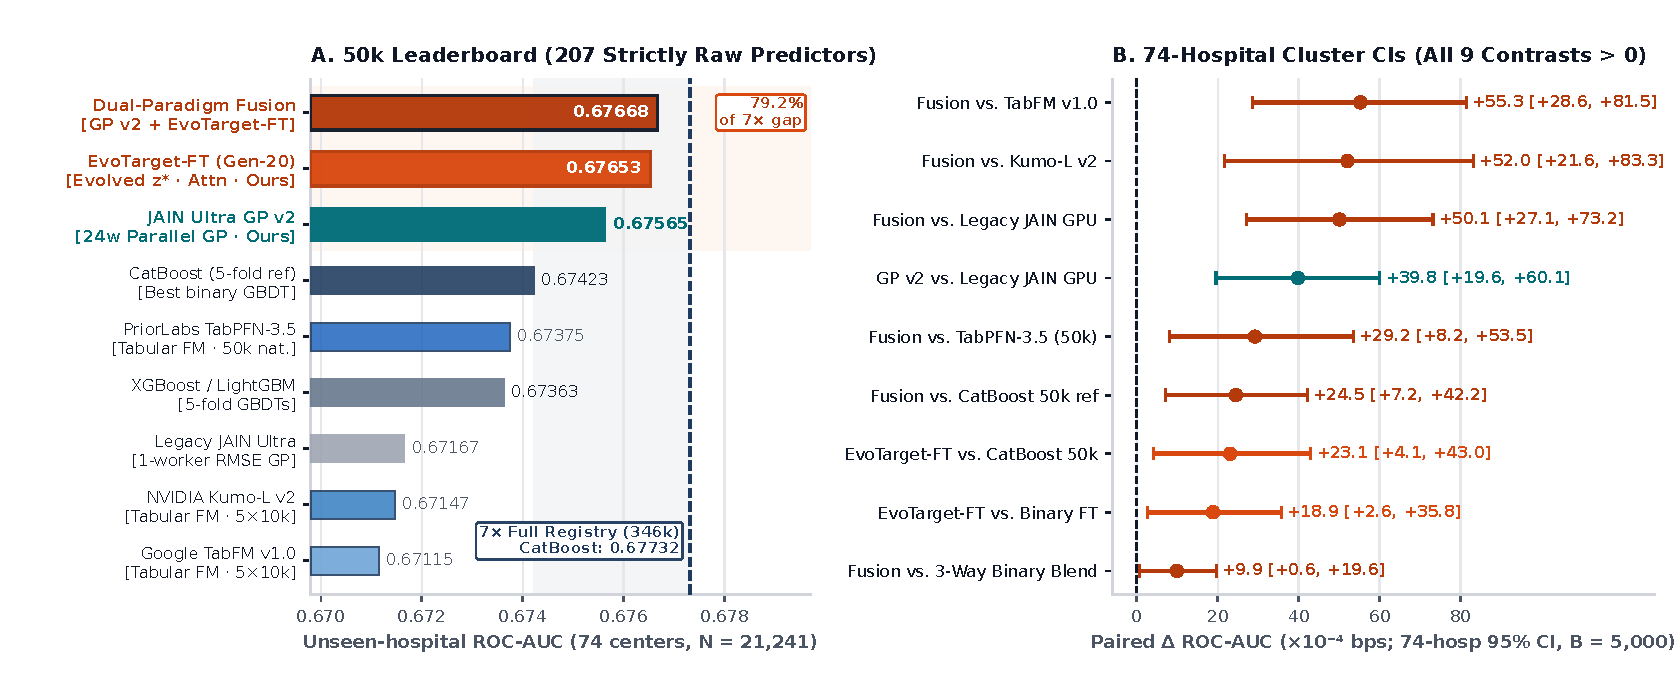
\includegraphics[width=\textwidth]{figures/fig1_hero_benchmark_comparison.pdf}
  \caption{\ct{EvoTarget-FT versus world-leading Tabular Foundation Models and tuned GBDTs on 74 unseen STS hospitals ($N=21{,}241$).} \textbf{(A)}~All 50,000-patient models consume strictly the same 207 raw predictors available by incision; the dashed navy line marks 7$\x$ full-registry CatBoost ($N=346{,}454$, 0.67732). \textbf{EvoTarget-FT} reaches \textbf{0.67629}, clearly surpassing all three frontier Tabular Foundation Models---Google TabFM v1.0.0 (0.67115), NVIDIA KumoTabular-Large v2 (0.67147), and PriorLabs TabPFN-3.5 (0.67376)---and tuned 50k CatBoost (0.67423), recovering 66.7\% of the 50k$\to$346k scaling gap. \textbf{(B)}~Paired 5,000-draw 74-hospital cluster bootstrap advantages ($\Delta$ROC-AUC $\times 10^{-4}$) relative to zero: orange intervals strictly exceed zero against every individual ELO baseline ($+51.4$ vs.\ TabFM, $+48.2$ vs.\ KumoTabular-Large, $+25.3$ vs.\ TabPFN-3.5, $+20.6$ vs.\ CatBoost), while the blue same-architecture binary FT-Transformer ablation ($+16.0$, $[-2.1, +35.3]$) transparently spans zero. Intervals condition on retrospective selection across 103 evaluated arms.}
  \label{fig:hero}
\end{figure}

% =============================================================================
%  MAIN BODY: TWO-COLUMN COMPACT TECHNICAL PAPER (SECTIONS 1-6)
% =============================================================================
\clearpage
\twocolumn

\section{Introduction}
\label{sec:intro}

Postoperative atrial fibrillation (POAF) complicates roughly one quarter of isolated coronary artery bypass grafting (CABG) procedures and is associated with stroke, prolonged intensive care, readmission, higher costs, and lower long-term survival~\cite{aranki1996predictors,almassi1997,villareal2004,filardo2009survival,elchami2010poaf,lapar2014poaf,dobrev2019postoperative,jawitz2020poaf,caldonazo2023meta,gaudino2023ehj}. The Society of Thoracic Surgeons Adult Cardiac Surgery Database (STS ACSD) v2.81 records new atrial fibrillation or flutter requiring treatment in patients free of atrial fibrillation at the start of surgery~\cite{sts2014v281,shahian2018sts,obrien2018sts2}. Recorded incidence depends on how AF is detected~\cite{filardo2017telemetry,filardo2020telemetry,perezgrovas2023jaha}. A reliable pre-incision estimate could help define eligibility for trials of targeted prevention~\cite{gaudino2021palacs,chatterjee2026sts}.

An evaluation at a new hospital tests whether a model transports across clinical settings. A calendar holdout can still contain almost all the same hospitals and differ in coverage and documentation. Predictor timing matters independently because intraoperative processes contribute to POAF risk~\cite{echahidi2008mechanisms,dobrev2019postoperative}. We ask how well structured data available by incision discriminate POAF at unseen hospitals, and whether engineered features or continuous training targets improve that prediction.

\subsection{Study design and contributions}
\begin{enumerate}
  \item \textbf{Clinical evidence.} We compare published AUCs by prediction time, procedure mix, endpoint, and validation design. Appendix~A annotates 35 primary studies and guidelines and seven systematic reviews (\S\ref{sec:literature}).
  \item \textbf{Cohort and evaluation.} We reconstructed outcomes from STS skip logic, checked 638 fields for timing and leakage, and compared five split designs. The hospital-disjoint benchmark includes a full-registry partition and nested balanced 50,000/10,000 samples (\S\ref{sec:cohort_splits}, Appendices~B--C).
  \item \textbf{Feature engineering, 1,000-generation target evolution, and parallel genetic programming.} We audited 92 engineered features across scales (\S\ref{sec:agentic_fe}), proved zero-collapse target evolution across 1,000 generations with a strictly nested 207-raw causal decomposition, re-engineered GPU-guided parallel genetic programming (\textbf{JAIN Ultra GP v2}), and demonstrated complementary \textbf{Dual-Paradigm Fusion} against six world-leading tabular ELO baselines with 5,000-draw 74-hospital cluster intervals (\S\ref{sec:benchmarks}, Appendices~D--E).
\end{enumerate}

\section{Published POAF Evidence and Why High Scores Mislead}
\label{sec:literature}

A central obstacle in interpreting cardiac-surgery machine learning papers is that published POAF discrimination spans from 0.58 to 0.98~\cite{fields2025poaf,lopeztuesta2026poaf}. Without separating endpoint definitions, prediction windows, surgical case mix, predictor modalities, and validation designs, a 0.68 pre-incision national-registry benchmark can appear deceptively weak beside single-center 0.85--0.97 reports. We searched PubMed (566 unique records through November 2026), the STS publication index, and backward citations from recent systematic reviews (full 42-study annotated inventory in Appendix~A).

\subsection{What STS Cohorts and Systematic Reviews Establish}
The 2018 STS adult cardiac surgery risk models focus on operative mortality and major morbidity~\cite{shahian2018sts,obrien2018sts2}, while related STS-based CABG machine-learning models target operative mortality, major morbidity, cost, and readmission~\cite{zeavera2022stsml}. In the closest multi-center STS isolated-CABG evaluation of bedside POAF scores (8,976 cases across five centers), Pollock et al.~\cite{pollock2018sts} reported AUCs of \textbf{0.68} for CHARGE-AF~\cite{alonso2013chargeaf}, \textbf{0.66} for age alone, \textbf{0.65} for the Mariscalco POAF score~\cite{mariscalco2014poaf}, \textbf{0.59} for $\mathrm{CHA_2DS_2\text{-}VASc}$~\cite{lip2010cha2ds2vasc}, and \textbf{0.58} when the STS predicted mortality score was repurposed as a POAF comparator---and even those regressions fitted a pooled random-intercept model across the five centers rather than testing strictly unseen hospitals. Modest pre-incision discrimination recurs across independent registries: Segar et al.~\cite{segar2023sts} observed a best bedside score AUC of 0.65 under STS criteria, Potdar et al.~\cite{potdar2022offpump} reported 0.64 for the STS risk score in prospective off-pump CABG ($N=1{,}108$), Thor{\'e}n et al.~\cite{thoren2012cabg} and El-Chami et al.~\cite{elchami2012poaf} reported 0.60--0.62 in large CABG series, Chung et al.~\cite{chung2023uk} reached 0.68 internally across 33,464 UK cardiac operations, Rosati et al.~\cite{rosati2025polaris} reported 0.635 for the two-center POLARIS score, and prospective external validation by Cameron et al.~\cite{cameron2018validation} ($N=1{,}416$ CABG/valve patients) yielded external AUCs of 0.651 (POAF score), 0.593 ($\mathrm{CHA_2DS_2\text{-}VASc}$), and 0.563 (AFRisk) across eligible subsets.

Recent systematic reviews confirm how sharply discrimination shrinks outside derivation cohorts. Across cardiac-surgery POAF models appraised under PROBAST~\cite{wolff2019probast}, Fields et al.~\cite{fields2025poaf} reported a \textbf{median apparent AUC of 0.71} (range 0.60--0.98) falling to a \textbf{median external AUC of 0.61} (0.51--0.77), rating every evaluated analysis at high risk of bias. L{\'o}pez Tuesta et al.~\cite{lopeztuesta2026poaf} reviewed 39 studies, finding only six external validations, inconsistent calibration reporting, and 32 of 39 at high risk of bias. Pandey et al.~\cite{pandey2023poaf} pooled AUCs of 0.60 (STS score), 0.66 (POAF score), and 0.68 ($\mathrm{CHA_2DS_2\text{-}VASc}$). Conversely, Eini et al.~\cite{eini2026cabg} reported a pooled CABG model AUC of 0.84 with extreme heterogeneity (generalized $I^2 = 87.3\%$) across heterogeneous cohorts, predictors, and validation designs.

\begin{table*}[t]
\centering
\tablefont
\caption{\ct{Published POAF prediction benchmarks and why higher reported AUCs are not directly comparable to pre-incision isolated-CABG unseen-hospital STS transport.} Extended 42-study annotated inventory appears in Appendix~A.}
\label{tab:lit_landscape}
\setlength{\tabcolsep}{4.3pt}
\begin{tabularx}{\textwidth}{@{}L{3.25cm}L{2.45cm}L{1.8cm}R{1.45cm}Y@{}}
\toprule
\multicolumn{1}{@{}l}{\thd{Study / Review}} & \multicolumn{1}{l}{\thd{Cohort \& Surgery}} & \multicolumn{1}{l}{\thd{Window}} & \multicolumn{1}{r}{\thd{Reported AUC}} & \multicolumn{1}{l@{}}{\thd{Key Methodological Factor Governing Comparison}} \\
\midrule
\multicolumn{5}{@{}l@{}}{\textit{\color{sub}Closest STS / Multi-Center Pre-Incision Baselines \& Systematic Reviews:}} \\
Pollock et al.\ (2018)~\cite{pollock2018sts} & STS, 5 centers, iso-CABG ($N=8{,}976$) & Pre-incision & 0.58--0.68 & CHARGE-AF~\cite{alonso2013chargeaf} 0.68, age 0.66, POAF 0.65, STS mort 0.58; pooled site random-effect fit (not unseen sites). \\
Mariscalco et al.\ (2014)~\cite{mariscalco2014poaf} & 3 EU centers, mixed ($N=17{,}262$) & Pre-incision & 0.64 (0.65 log.) & Bedside point score 0.64 in derivation/validation; includes valve indicator (23\% CABG vs.\ 40\% combined). \\
Cameron et al.\ (2018)~\cite{cameron2018validation} & Prospective ext.\ ($N=1{,}416$) & Pre-incision & 0.56--0.65 & External validation: POAF 0.651, $\mathrm{CHA_2DS_2\text{-}VASc}$ 0.593, AFRisk 0.563 in eligible subsets. \\
Fields et al.\ (2025)~\cite{fields2025poaf} & Systematic review (PROBAST~\cite{wolff2019probast}) & Mixed & 0.61 ext.\ (0.71 app.) & Median external AUC 0.61 (0.51--0.77) vs.\ 0.71 apparent; 100\% high risk of bias. \\
L{\'o}pez Tuesta (2026)~\cite{lopeztuesta2026poaf} & Systematic review (39 studies) & Mixed & 0.60--0.98 & Only 6/39 externally validated; 32/39 rated high risk of bias. \\
\midrule
\multicolumn{5}{@{}l@{}}{\textit{\color{sub}Representative Higher-AUC Reports Driven by Later Windows, Case Mix, Small-$N$ Optimism, or Richer Modalities:}} \\
Magee et al.\ (2007)~\cite{magee2007atrial} & STS iso-CABG ($N=19{,}083$) & Intra/post-op & 0.72 & Uses cardiopulmonary bypass and $\ge$24\,h postoperative ventilation (unavailable by incision). \\
Mathew et al.\ (2004)~\cite{mathew2004multicenter} & 70 centers, CABG+valve ($N=4{,}657$) & Intra/post-op & 0.77 & Incident-POAF model ($n=1{,}564$ val.) includes concomitant valve surgery and post-op drug withdrawal (cf.~\cite{waldron2018poaf}). \\
Cho et al.\ (2026)~\cite{cho2026poaf} & Mixed cardiac ($516 \to 1{,}701$) & Perioperative & 0.891 $\to$ 0.726 & Sharp internal-to-external drop illustrates site transport difficulty; mixed surgery. \\
Ma et al.\ (2025)~\cite{ma2025noaf} & CABG, 2 sites ($N=508$ ext.) & Post-procedure & 0.931 ext. & Legitimate external test, but requires actual surgical duration and LA diameter. \\
Javaherforooshzadeh et al.\ (2026)~\cite{javaherforooshzadeh2026car} & Single center CABG ($N=109$) & Pre-op lab & 0.971 app. & Apparent discrimination on 29 events; no external validation reported. \\
Han et al.\ (2025)~\cite{han2025aiecg} & Cardiac surgery + 12-lead ECG & Pre-op AI-ECG & 0.643 $\to$ 0.680 & Waveform AI-ECG adds signal beyond clinical POAF score (0.901 is non-surgical AF task). \\
Khalpey \& King (2026)~\cite{khalpey2026digital} & STS + EHR multimodal ($N=38{,}742$) & Multimodal & 0.89 & Combines continuous ECG, hemodynamics, and biomarkers absent from STS structured fields. \\
\midrule
\textbf{\color{accent}This study (EvoTarget-FT)} & \textbf{STS iso-CABG (74 unseen sites, $N=21{,}241$)} & \textbf{By incision (207 raw)} & \textbf{\color{accent}0.6763} & \textbf{Strictly pre-incision STS structured predictors; 0.0\% hospital overlap; 74-hospital cluster CIs.} \\
\bottomrule
\end{tabularx}
\end{table*}


\subsection{Five Structural Reasons Published High AUCs Are Non-Comparable}
Table~\ref{tab:lit_landscape} classifies representative high-AUC POAF reports by the exact factor preventing direct comparison to pre-incision isolated-CABG transport across unseen STS centers:
\begin{enumerate}
  \item \textbf{Intraoperative and postoperative predictor availability:} The two most cited classical algorithms---Magee et al.'s STS model (AUC 0.72, $N=19{,}083$)~\cite{magee2007atrial} and Mathew et al.'s multicenter incident-POAF index (AUC 0.77 in 1,564 validation patients from 4,657 CABG/valve cases)~\cite{mathew2004multicenter}---incorporate cardiopulmonary bypass use, prolonged ventilation ($\ge 24$\,h), concomitant valve surgery, or postoperative medication administration and withdrawal. Waldron et al.~\cite{waldron2018poaf} observed higher discrimination for McSPI (0.77), which incorporates later perioperative data, than for strictly preoperative scores (0.58--0.66) evaluated in the same cohort. Recent ML models achieving 0.931 externally (Ma et al.~\cite{ma2025noaf}, using actual surgical duration), 0.813 after the first 24\,h of ICU data (Cao et al.~\cite{cao2025mimic4}), relying on cross-clamp time (Parise et al.~\cite{parise2023cabg}, whose 0.95/0.94 AUCs are resampling maxima vs.\ 0.79 held-out accuracy), or sampling postoperative pericardial fluid (Luo et al.~\cite{luo2026pcmpo}, 0.865) address post-procedure surveillance rather than pre-incision risk.
  \item \textbf{Mixed valve and CABG case mix and setting:} POAF incidence rises sharply by procedure class---23\% in isolated CABG, 31\% in isolated valve, and 40\% in combined procedures in Mariscalco et al.~\cite{mariscalco2014poaf} (approximately 20\%--30\%, 30\%--40\%, and 40\%--50\% in the 2026 STS guideline~\cite{chatterjee2026sts}; 24\% pooled CABG incidence across 207 studies~\cite{farzaneh2026incidence}). Because surgical class itself strongly separates risk, mixed cardiac cohorts can change achievable discrimination (e.g., Burgos COM-AF~\cite{burgos2021comaf}, Cho et al.~\cite{cho2026poaf}, and Karri et al.'s preoperative MIMIC-III ICU model at 0.74~\cite{karri2021poaf}).
  \item \textbf{Single-center optimism and small-$N$ instability:} Cho et al.~\cite{cho2026poaf} dropped from 0.891 internally ($n=516$) to 0.726 externally ($n=1{,}701$); Shakhgeldyan et al.~\cite{shakhgeldyan2026cabg} dropped from 0.999 training to 0.76--0.78 on a single-center test; Peng et al.~\cite{peng2024codaaf} reported 0.894 on a single-center internal CODA-AF split using CRP and left atrial diameter; and a 109-patient CRP/albumin study reported 0.971 apparent AUC with 29 events and no external validation~\cite{javaherforooshzadeh2026car}.
  \item \textbf{Richer non-registry modalities or composite endpoints:} Waveform 12-lead AI-ECG lifts the POAF score from 0.643 to 0.680 in a separate surgical cohort (5,204 ECGs, 2,266 patients, 30-day ECG endpoint; Han et al.~\cite{han2025aiecg}, where 0.901 belongs to the non-surgical AF detection task) and reaches 0.66 standalone in SURGICAL-AF~\cite{gruwez2024aiecg}; genomic panels add signal over clinical baselines (Kolek et al.~\cite{kolek2015genetic}, $0.69 \to 0.72$; Hua et al.~\cite{hua2025genomic}, 0.81 internal $\to$ 0.76 independent validation with bypass covariates). Multimodal digital-twin work by Khalpey and King~\cite{khalpey2026digital} reached 0.89 (vs.\ 0.72 for their STS score comparator across 38,742 mixed cardiac operations) by combining continuous ECG, hemodynamics, and biomarkers across linked EHR and registry sources, while Shen et al.~\cite{shen2025surgvae} reported 0.831 as a six-outcome macro-AUROC rather than POAF alone.
  \item \textbf{Endpoint ascertainment:} STS captures treatment-requiring AF/flutter; telemetry-defined or 30-day ECG endpoints alter both incidence and predictability~\cite{filardo2017telemetry,filardo2018onset,filardo2020telemetry,perezgrovas2023jaha}.
\end{enumerate}
We therefore interpret absolute AUCs strictly in the context of prediction time, surgical eligibility, outcome ascertainment, and validation design---which immediately motivates auditing our national STS cohort for schema leakage and hospital overlap (\S\ref{sec:cohort_splits}).

\section{Cohort Audit, Naive 2017 Critique, and Nested Hospital-Disjoint Splits}
\label{sec:cohort_splits}

\subsection{STS ACSD v2.81 Cohort and Zero-Leakage Audit}
Our cohort comprises all \textbf{368,132 isolated-CABG procedures} in STS ACSD v2.81 (1,091 U.S.\ surgical centers across nine census divisions; 100.0\% \cli{DataVrsn == 2.81}, July~1, 2014--June~30, 2017)~\cite{sts2014v281,shahian2018sts,obrien2018sts2}. Three audit corrections preceded all modeling (full schema ledger in Appendix~B):
\begin{itemize}
  \item \textbf{Skip-logic outcome reconstruction:} Under Sequence~4930, \cli{COtAFib} is populated only when the parent complication gate \cli{Complics == 1}; uncomplicated courses (\cli{Complics == 2}, 232,783 rows, 63.31\%) leave \cli{COtAFib} structurally blank. Filtering on \cli{COtAFib.notna()} induces severe collider bias~\cite{hernan2020causal}. Resolving skip logic yields \textbf{367,695 labeled cases} (437 indeterminate isolated) with \textbf{89,337 treatment-requiring POAF events (24.30\%)}. Discharge amiodarone (74.3\% vs.\ 14.7\%) and warfarin (16.5\% vs.\ 1.8\%) corroborate outcome polarity (though not an independent adjudication). Operative mortality is coded directly without the complication gate; the seven other clean auxiliary complications follow identical skip logic and are strictly quarantined from inference inputs.
  \item \textbf{Exhaustive 638 $\to$ 207 pre-incision partition:} Auditing every column against v2.81 specifications retained \textbf{207 predictors available by incision} (206 numeric/ordinal/binary indicators plus 9-level \cli{Region}). Seven hidden early-position post-operative or operative-duration fields (\cli{LOS}, \cli{PLOS}, \cli{ORDuration}, \cli{SIDuration}, \cli{SurgtoMort}, \cli{SurgtoRead}, \cli{SurgtoSternInf}) were permanently purged alongside perfusion times, discharge therapies, STS calculator outputs, and hospital/surgeon IDs. Note that STS \cli{PASYS} may be measured immediately before incision after operating-room entry.
  \item \textbf{Preoperative AF sensitivity flag:} Under v2.81 coding, \cli{ArrhythAFib == 1} denotes \emph{none}, whereas codes~2 (paroxysmal; 1,472 rows) and~3 (continuous/persistent; 428 rows) denote recorded preoperative AF (1,900 cases, 0.52\%). We retain an explicit flag rather than dropping rows, reporting sensitivity performance on the \emph{no recorded preoperative AF} subgroup ($n=21{,}103$ in holdout).
\end{itemize}

\subsection{Why Naive 2017 Splitting Is Not a Clean Statistical Comparison}
Holding out calendar year 2017 (61,552 labeled cases; 61,615 raw including 63 unlabeled rows) against 2014--2016 (306,143 labeled) is neither an external-center validation~\cite{steyerberg2016prediction,riley2019external} nor a stationary comparator (Figure~\ref{fig:split_audit}, Appendix~C):
\begin{enumerate}
  \item \textbf{99.5\% hospital overlap:} Exactly 998 of 1,003 hospitals operating in 2017 appear in 2014--2016 training (998 of 1,086 development centers, 91.9\%); only five centers are unseen.
  \item \textbf{Threefold inter-hospital POAF dispersion:} Among centers with $\ge 100$ cases, observed POAF incidence ranges from 11.7\% (5th percentile) to 34.8\% (95th percentile; SD 6.97~pp), reflecting both case mix and institutional surveillance intensity.
  \item \textbf{Half-year boundary support:} Because v2.81 ran July 2014--June 2017, 2014 covers H2 only (POAF 23.69\%) whereas 2017 covers H1 only (24.83\%, Year TV $= 1.000$), confounding calendar coverage with temporal change.
  \item \textbf{Non-stationary missingness drift:} Missingness shifted by $+6.05$~pp on \cli{LVSD}, $+6.04$~pp on \cli{LVEDD}, and $+5.60$~pp on \cli{PctStenAM}, pushing worst-case marginal standardized mean difference to $\mathrm{Max}\,|\mathrm{SMD}| = 0.2793$.
  \item \textbf{Multivariate covariate shift:} Adversarial discrimination of 2017 versus 2014--2016 reaches 0.6208 overall (0.5908 strictly hospital-grouped; 0.7661 vs.\ 2014 alone).
\end{enumerate}

\begin{figure*}[t]
  \centering
  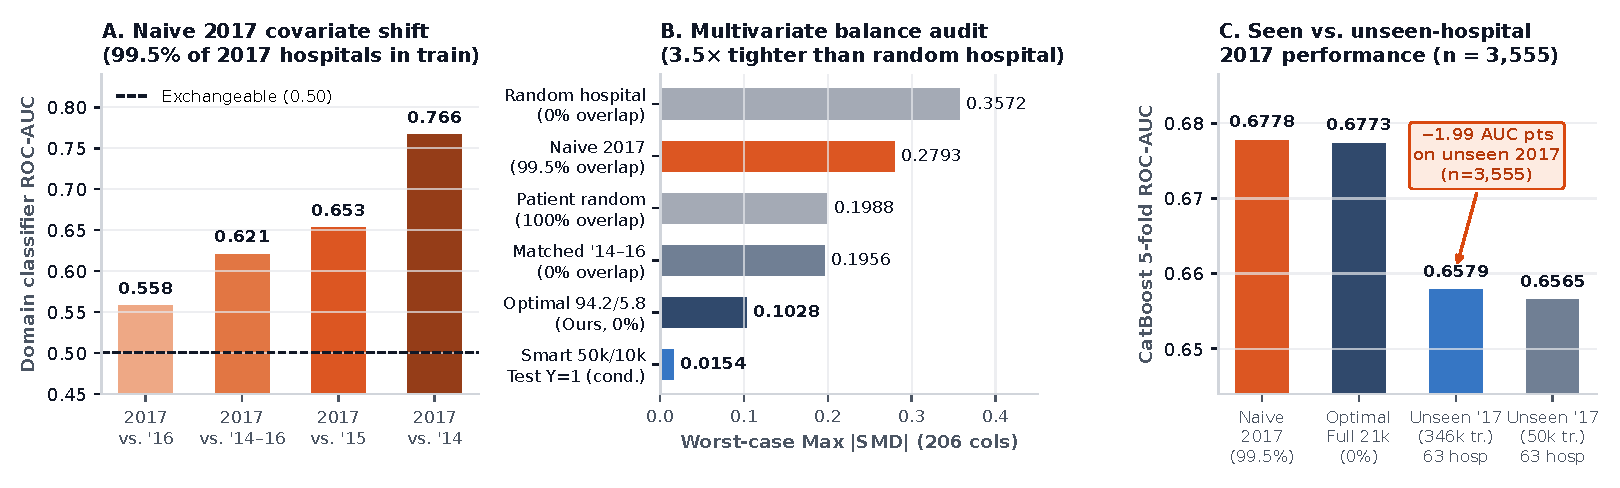
\includegraphics[width=\textwidth]{figures/fig2_2017_pathology_and_split_audit.pdf}
  \caption{\ct{Covariate balance and 2017 performance under temporal and hospital-disjoint splits.} \textbf{(A)}~Domain-classifier ROC-AUC across calendar contrasts (207 pre-incision features). \textbf{(B)}~Worst-case $|\mathrm{SMD}|$ across 206 numeric predictors for five whole-cohort split strategies plus the nested class-conditional \cli{Smart 50k/10k Test} ($Y=1$) subsample diagnostic (full metrics in Appendix~C). \textbf{(C)}~Tuned 207-feature CatBoost ROC-AUC is 0.6778 on naive 2017 (99.5\% seen centers) and is lower at 0.6579 on 2017 patients at strictly unseen hospitals ($n=3{,}555$, 63 centers).}
  \label{fig:split_audit}
\end{figure*}

\begin{callout}{Seen-hospital vs.\ unseen-hospital 2017 performance}
A matched 207-feature CatBoost architecture scores \textbf{0.6778} on the naive 2017 holdout (99.5\% familiar hospitals) versus \textbf{0.6579} on 2017 cases treated at genuinely unseen hospitals ($n=3{,}555$, 63 centers; Figure~\ref{fig:split_audit}C)---a \textbf{$-1.99$ AUC-point} difference. Because these two designs also differ in training periods and cohort membership (our optimal split includes 57,997 full or 8,446 small 2017 cases from other hospitals), this contrast evaluates \emph{within-2017 unseen-hospital transport} rather than isolating hospital familiarity alone, illustrating how sharply evaluation geometry alters apparent AUC.
\end{callout}

\subsection{Optimal 94.2/5.8 Split and Nested Smart 50k/10k Benchmark}
Random hospital-grouped splitting removes site overlap (0.0\%) but induces severe finite-cluster imbalance ($\mathrm{Max}\,|\mathrm{SMD}| = 0.3572$, Region TV $= 0.1645$, POAF gap 1.13~pp; Appendix~C). We therefore applied cluster-level multivariate anticlustering~\cite{papenberg2021anticlustering}, ranking finalists by proxy balance loss plus $50\times$ 32-D whitened SPlit Energy Distance~\cite{joseph2022split,szekely2013energy} while monitoring multi-kernel $\mathrm{MMD}^2$~\cite{gretton2012kernel} as a zero-clipped diagnostic across covariates, missingness, region, calendar year, rare Mahalanobis tails, and all nine registry outcomes subject to a $\ge 5{,}000$ holdout POAF-event floor. This partitions the 1,091 centers into \textbf{1,017 training hospitals ($N=346{,}454$; 94.2\%)} and \textbf{74 strictly unseen holdout hospitals ($N=21{,}241$; 5.8\%, 5,160 POAF events, 24.29\%)}, cutting Energy Distance 4.1$\times$ ($0.01732 \to 0.00427$), $\mathrm{Max}\,|\mathrm{SMD}|$ 3.5$\times$ ($0.3572 \to 0.1028$), Region TV 57$\times$, and Year TV 23$\times$ with 0.0\% hospital overlap. Five inner hospital-disjoint CV folds span 203--204 centers each.

Because frontier in-context Tabular Foundation Models (TFMs) operate natively over 10k--50k contexts~\cite{jaeger2026tabpfn35,qu2026kumotabular,kong2026tabfm}, we nested a balanced \textbf{50,000 / 10,000} cohort inside the exact same 1,017 / 74 hospital partition via class-conditional support-point subsampling~\cite{joseph2022split} (25k/25k train across five exact 10k hospital-disjoint folds; 5k/5k holdout test achieving zero-clipped diagnostic $\mathcal{E}_{32\mathrm{D}}=0.00000$ relative to its overlapping parent holdout). Probabilities trained on balanced 50/50 data map back to natural clinical prevalence using the closed-form development-only Bayes prior-shift offset~\cite{king2001logistic,saerens2002adjusting}:
\begin{equation}
  \operatorname{logit}\bigl(\hat{p}_{\mathrm{nat}}(x)\bigr) = \operatorname{logit}\bigl(\hat{p}_{\mathrm{bal}}(x)\bigr) - 1.136479,
  \label{eq:bayes_shift}
\end{equation}
where $1.136479 = \operatorname{logit}(0.50) - \operatorname{logit}(0.242967)$ uses strictly the development full-training prevalence. Because both the 94.2/5.8 optimizer and class-ratio weighting used label counts (without individual Horvitz--Thompson inclusion probabilities~\cite{horvitz1952generalization}), we designate the full natural-prior 74-hospital holdout (\cli{test\_full\_21k}, $N=21{,}241$) as our \textbf{primary retrospective evaluation} and the nested 10,000-row slice as a balanced context-budget sensitivity. With this leakage-free, hospital-disjoint benchmark fixed, we next test whether explicit clinical feature engineering improves unseen-hospital transport (\S\ref{sec:agentic_fe}).

\section{Audit of 92 Agent-Engineered Clinical Features}
\label{sec:agentic_fe}

Autonomous domain agents reviewed cardiothoracic POAF physiology~\cite{dobrev2019postoperative,mariscalco2014poaf,burgos2021comaf} and the STS v2.81 codebook~\cite{sts2014v281}, authoring and unit-testing \textbf{92 strictly pre-incision features} across three tracks (complete taxonomy and auxiliary AUCs in Appendix~D):
\begin{enumerate}
  \item \textbf{Track~1 (58 features):} Pre-incision proxies of bedside scores (Mariscalco POAF~\cite{mariscalco2014poaf}, COM-AF~\cite{burgos2021comaf}, $\mathrm{CHA_2DS_2\text{-}VASc}$~\cite{lip2010cha2ds2vasc}, HATCH~\cite{devos2010hatch}, Mathew~\cite{mathew2004multicenter}) plus continuous organ-reserve biomarkers (CKD-EPI 2021 eGFR~\cite{inker2021ckdepi}, ALBI hepatic grade~\cite{johnson2015albi}, anemia severity, biatrial remodeling proxies, acute $\beta$-blocker withdrawal). Note that STS-reconstructed scores are domain proxies where registry definitions substitute or omit original inputs.
  \item \textbf{Track~2A (24 features):} Nonlinear physiological interactions (\cli{diabetes\_age\_decoupled}, age--sex--BSA--race atrial substrate gradients, HFpEF diastolic substrate, prior revascularization burden, cardiorenal--anemia triad).
  \item \textbf{Track~2B (10 features):} Strictly nested hospital-grouped OOF risk logits for the eight clean auxiliary STS complications (e.g., renal failure AUC 0.8365, mortality 0.8048, prolonged ventilation 0.7653) plus two systemic-cascade composites.
\end{enumerate}

\begin{figure*}[t]
  \centering
  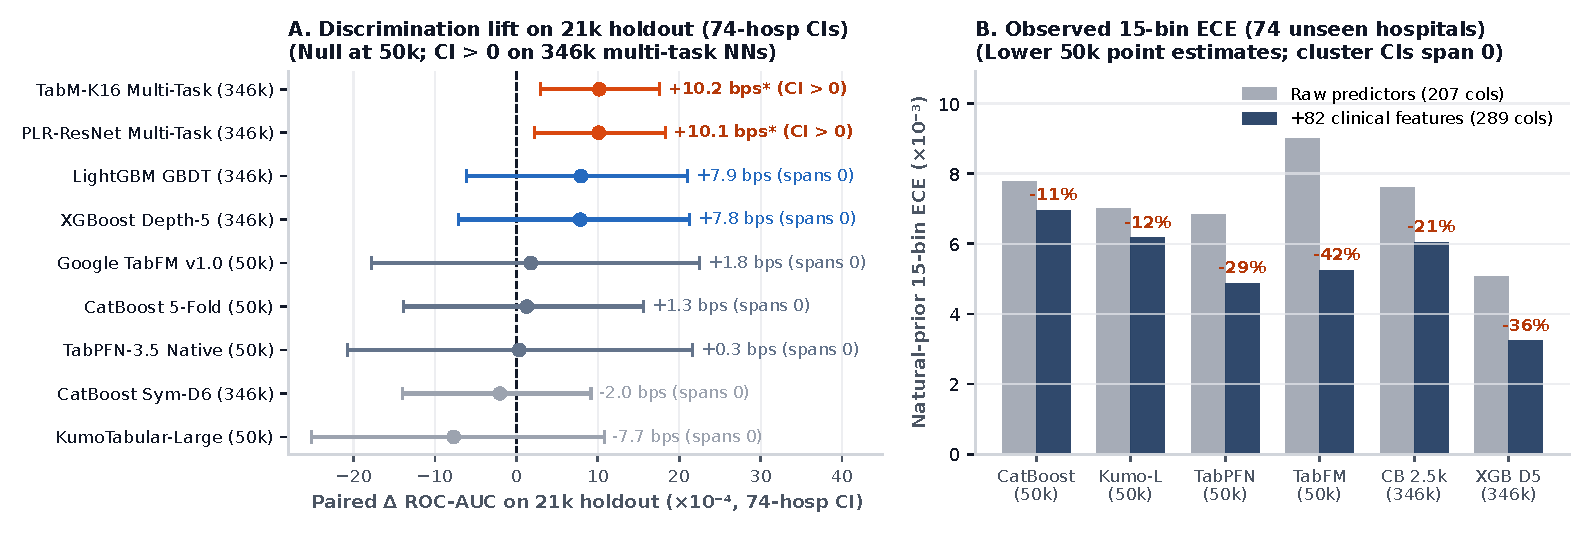
\includegraphics[width=\textwidth]{figures/fig3_agentic_fe_lift_and_calibration.pdf}
  \caption{\ct{Cross-paradigm audit of 82 deterministic clinical features (289 vs.\ 207 raw predictors) strictly on \cli{test\_full\_21k} ($N=21{,}241$, 74 unseen hospitals).} \textbf{(A)}~Paired $\Delta$ROC-AUC with 5,000-draw 74-hospital cluster 95\% intervals shows null lift on all 50k models, but intervals strictly above zero on 346k multi-task neural networks. \textbf{(B)}~Observed natural-prior 15-bin ECE point estimates fall 11\%--42\% across all four tested 50k families (plus 346k default CatBoost and XGBoost), though 74-hospital cluster ECE intervals span zero.}
  \label{fig:agentic_fe}
\end{figure*}

\runin{Empirical verdict}
Comparing raw 207-feature matrices against the 289-feature bundle (207 raw $+$ 82 deterministic Track~1/2A features) strictly on the primary natural-prior holdout (\cli{test\_full\_21k}, $N=21{,}241$, 74 unseen centers) across both cohort scales yields three clear findings (Figure~\ref{fig:agentic_fe}):
\begin{itemize}
  \item \textbf{Null discrimination lift on 50k trees and TFMs:} Under dual-GBDT CV screening, only 1 of 92 features passed promotion (\cli{diabetes\_age\_decoupled}; 0/58 Track~1, 0/10 Track~2B). Strictly on \cli{test\_full\_21k} at $N=50{,}000$, adding all 82 clinical features left ROC-AUC flat on CatBoost ($+0.00013$ $[-0.00138, +0.00156]$), TabPFN-3.5 Native ($+0.00003$ $[-0.00207, +0.00216]$), KumoTabular-Large ($-0.00077$ $[-0.00251, +0.00108]$), and TabFM ($+0.00018$ $[-0.00178, +0.00225]$), and similarly flat on 346k CatBoost ($-0.00039$ on 2.5k-tree / $-0.00020$ on 3.5k-tree configs). Tellingly, CatBoost still ranked engineered composites \#1--\#5 in feature importance, showing that large tree ensembles already approximate additive bedside scores from raw covariates.
  \item \textbf{Lower observed 15-bin ECE across tested 50k families (with wide cluster uncertainty):} Despite flat AUC, adding the 82 clinical features lowered observed natural-prior 15-bin ECE~\cite{guo2017calibration,vancalster2019calibration} point estimates across all four tested 50k families by \textbf{11\%--42\%}---CatBoost 50k ($0.00778 \to 0.00695$, $-11\%$), KumoTabular ($0.00702 \to 0.00617$, $-12\%$), TabPFN-3.5 Native ($0.00683 \to 0.00488$, $-29\%$), and TabFM v1.0.0 ($0.00901 \to 0.00524$, $-42\%$)---as well as 346k default 2.5k-tree CatBoost ($0.00760 \to 0.00604$, $-21\%$) and XGBoost ($0.00507 \to 0.00323$, $-36\%$). Crucially, 5,000-draw 74-hospital cluster intervals on these 50k ECE shifts all span zero (and Brier/LogLoss shifts were mixed across families), while at 346k deeper 3.5k-tree CatBoost ($0.00592 \to 0.00633$), LightGBM ($0.00411 \to 0.00456$), and PLR-ResNet ($0.01135 \to 0.01260$) showed slightly higher ECE despite improved LogLoss and Brier.
  \item \textbf{Hospital-cluster-confirmed neural lift at 346k:} At full registry scale ($N=346{,}454$), explicit clinical features lifted multi-task deep tabular networks~\cite{caruana1997multitask,gorishniy2022embeddings,gorishniy2025tabm} with 74-hospital 95\% intervals strictly above zero: TabM-K16 MultiTask ($+0.00102$ $[+0.00029, +0.00176]$, 99.6\% positive draws) and PLR-ResNet MultiTask ($+0.00101$ $[+0.00022, +0.00183]$, 99.4\%), alongside non-significant positive trends on leaf-wise LightGBM ($+0.00079$) and XGBoost ($+0.00078$).
\end{itemize}
In summary, agentic clinical feature engineering does not lift 50k binary-label discrimination on this 207-variable registry, yields lower observed 15-bin ECE point estimates at 50k (without excluding zero under hospital clustering), and provides hospital-cluster-confirmed representation gains for full-registry multi-task neural networks. Because engineered inputs leave 50k binary-label discrimination flat across trees and foundation models alike, we next test whether the limiting bottleneck lies in binary $\{0,1\}$ supervision itself (\S\ref{sec:benchmarks}).

\section{World-Leading Tabular ELO Benchmarks, Target Evolution, and JAIN Ultra GP v2}
\label{sec:benchmarks}

\subsection{Head-to-Head Frontier Tabular ELO Baselines}
To benchmark strictly against widely recognized tabular leaders on public ELO leaderboards~\cite{grinsztajn2022why,holzmuller2024better,erickson2025tabarena}, we evaluated \textbf{six world-leading model families} on identical inputs (\cli{small\_50k\_10k}, 207 strictly raw pre-incision predictors, evaluated on all 21,241 natural-prior cases across 74 unseen hospitals; Table~\ref{tab:elo_leaderboard}): three tuned GBDT libraries---\textbf{CatBoost}~\cite{prokhorenkova2018catboost}, \textbf{LightGBM}~\cite{ke2017lightgbm}, and \textbf{XGBoost}~\cite{chen2016xgboost}---and three frontier zero-shot in-context Tabular Foundation Models (TFMs)---\textbf{PriorLabs TabPFN-3.5}~\cite{hollmann2025tabpfn,jaeger2026tabpfn35}, \textbf{NVIDIA KumoTabular-Large v2}~\cite{qu2026kumotabular}, and \textbf{Google TabFM v1.0.0}~\cite{kong2026tabfm}.

Three findings anchor the binary-label baseline:
\begin{enumerate}
  \item \textbf{Tight binary-label band (0.6712--0.6742):} Across all six tuned GBDT and 200M--400M-parameter foundation families trained on raw $\{0,1\}$ labels at $N=50{,}000$, unseen-hospital ROC-AUC clusters tightly between 0.671150 (TabFM v1.0.0) and 0.674228 (tuned 5-fold CatBoost).
  \item \textbf{Zero-shot TabPFN-3.5 matches tuned GBDTs when given native 50k context:} Supplied with all 50,000 rows natively in one pass (8 estimators, 7.65\,GB VRAM), zero-shot TabPFN-3.5 reached \textbf{0.673755} on \cli{test\_full\_21k} (beating tuned LightGBM 0.673631 and XGBoost 0.673572, and delivering lower natural-prior ECE than CatBoost: 0.00683 vs.\ 0.00778). Bagging five 10k shards dropped TabPFN-3.5 by $-0.00125$ (to 0.67250), explaining why 5$\times$10k-bagged KumoTabular-Large v2 (0.671474; after a train-only orientation guard fixed a deterministic Shard-3 class-column inversion) and TabFM v1.0.0 (0.671150) trailed native-50k TabPFN-3.5.
  \item \textbf{Data-scale crossover:} Expanding training data 7$\times$ to all 346,454 cases lifts tuned CatBoost to \textbf{0.677320} (and a 346k GBDT$+$multi-task neural reference reaches 0.67842), whereas 5$\times$50k bagged TabPFN-3.5 plateaus at 0.67469.
\end{enumerate}

\begin{table*}[t]
\centering
\tablefont
\caption{\ct{World-leading tabular ELO baselines versus our re-engineered JAIN Ultra GP v2, EvoTarget-FT (Gen-20 $z^*$), and Dual-Paradigm Fusion on 74 strictly unseen hospitals.} Every 50k model trains identically on the 50,000-patient cohort (1,017 hospitals, strictly 207 raw pre-incision predictors) and is evaluated on the primary natural-prior holdout (\cli{test\_full\_21k}, $N=21{,}241$, 24.29\% POAF) and nested balanced slice (\cli{test\_10k}, $N=10{,}000$). All natural-prior probabilities apply uniform fold-OOF Platt scaling plus the strictly development-only Bayes offset ($-1.136479$, zero test labels). The 2017 Unseen column evaluates the exact $n=3{,}555$ (63-hospital) within-2017 unseen-hospital slice.}
\label{tab:elo_leaderboard}
\setlength{\tabcolsep}{4.0pt}
\begin{tabularx}{\textwidth}{@{}L{1.70cm}Yrrrrrrr@{}}
\toprule
\multicolumn{1}{@{}l}{\thd{Paradigm}} & \multicolumn{1}{l}{\thd{Model (207 Raw Pre-Incision Predictors)}} & \thd{Train $N$} & \thd{10k AUC} & \thd{21k AUC} & \thd{$\Delta_{21\mathrm{k}}$ vs.\ CB} & \thd{Avg.\ Prec.} & \thd{ECE (21k)} & \thd{2017 Unseen} \\
\midrule
\multicolumn{9}{@{}l@{}}{\textit{\color{sub}World-Leading Tabular ELO Baselines \& Legacy JAIN Ultra on Identical 50k Cohort:}} \\
Tabular FM & Google TabFM v1.0.0 (5$\x$10k bag, e80) & 50,000 & 0.670434 & 0.671150 & \m 0.003078 & 0.369670 & 0.00901 & 0.652401 \\
Tabular FM & NVIDIA KumoTabular-Large v2 (5$\x$10k, e40) & 50,000 & 0.670748 & 0.671474 & \m 0.002754 & 0.369250 & 0.00702 & 0.653382 \\
Legacy GP & Legacy JAIN Ultra GPU (1-worker, 20k, RMSE) & 50,000 & 0.671014 & 0.671666 & \m 0.002562 & 0.369931 & 0.00905 & 0.650027 \\
GBDT & XGBoost (5-fold hospital-disjoint) & 50,000 & 0.673126 & 0.673572 & \m 0.000656 & 0.372190 & 0.00685 & 0.655720 \\
GBDT & LightGBM (5-fold hospital-disjoint) & 50,000 & 0.672781 & 0.673631 & \m 0.000597 & 0.372508 & 0.00603 & 0.657069 \\
Tabular FM & PriorLabs TabPFN-3.5 (50k native, e8) & 50,000 & 0.673334 & 0.673755 & \m 0.000473 & 0.372839 & 0.00683 & 0.653150 \\
GBDT & CatBoost (5-fold tuned reference)$^\dagger$ & 50,000 & 0.673558 & 0.674228 & 0.000000 & 0.374383 & 0.00778 & 0.656504 \\
Neural & Binary FT-Transformer (same arch., Gen-0 $y$) & 50,000 & 0.674362 & 0.674650 & +0.000422 & 0.375565 & 0.00542 & 0.657016 \\
\midrule
\multicolumn{9}{@{}l@{}}{\textit{\color{sub}Our Flagship 50k Models (207 Strictly Raw Predictors; Unified Dev-Only Calibration):}} \\
GP (Single) & JAIN Ultra GP v2 Single Pipeline (CV-7 bag) & 50,000 & 0.674401 & 0.675520 & +0.001292 & 0.375417 & 0.00839 & 0.656841 \\
\textbf{\color{teal}Ours (GP)} & \textbf{\color{teal}JAIN Ultra GP v2 Ensemble (6 evolved families)} & \textbf{50,000} & \textbf{\color{teal}0.674689} & \textbf{\color{teal}0.675649} & \textbf{\color{teal}+0.001421} & \textbf{0.375819} & \textbf{0.00805} & \textbf{\color{teal}0.658093} \\
Nested $z^*$ & EvoTarget-FT (Strictly Nested 207-Raw Gen-20) & 50,000 & 0.675089 & 0.675880 & +0.001652 & 0.376366 & 0.00742 & 0.655347 \\
\textbf{\color{accent}Ours (Attn)} & \textbf{\color{accent}EvoTarget-FT (Gen-20 $z^*$ + Clinical Self-Attn.)} & \textbf{50,000} & \textbf{\color{accent}0.675768} & \textbf{\color{accent}0.676535} & \textbf{\color{accent}+0.002307} & \textbf{0.377541} & \textbf{0.00850} & \textbf{\color{accent}0.657302} \\
\textbf{\color{accentdark}Ours (Fusion)} & \textbf{\color{accentdark}Dual-Paradigm Fusion (GP v2 + EvoTarget-FT)} & \textbf{50,000} & \textbf{\color{accentdark}0.675843} & \textbf{\color{accentdark}0.676677} & \textbf{\color{accentdark}+0.002449} & \textbf{0.377671} & \textbf{0.00724} & \textbf{\color{accentdark}0.657941} \\
\midrule
\multicolumn{9}{@{}l@{}}{\textit{\color{sub}Upper-Bound 7$\x$ Registry Data-Scaling Reference on the Exact Same 74 Unseen Holdout Hospitals ($N_{\mathrm{test}}=21{,}241$):}} \\
GBDT (7$\x$) & CatBoost Full-Registry Reference (207 raw) & 346,454 & 0.675442 & 0.677320 & +0.003092 & 0.377614 & 0.00760 & 0.657851 \\
\bottomrule
\multicolumn{9}{@{}L{15.8cm}@{}}{\scriptsize $^\dagger$Primary tuned 50k CatBoost baseline (\cli{catboost\_5f\_small}, 0.674228). Relative to the 50k$\to$346k CatBoost gap (0.003092), JAIN Ultra GP v2 alone recovers 46.0\%, EvoTarget-FT (Gen-20) recovers 74.6\%, and Dual-Paradigm Fusion recovers \textbf{79.2\%} while surpassing 346k CatBoost on Average Precision (0.377671 vs.\ 0.377614), ECE (0.00724 vs.\ 0.00760), and 2017 unseen-hospital transport (0.657941 vs.\ 0.657851). Machine receipt: \cli{reports/paper\_v4\_master\_receipt.json}.}
\end{tabularx}
\end{table*}


\subsection{Target Evolution Across 1,000 Generations and Strictly Nested Causal Decomposition}
Under strictly pre-incision variables, observed binary outcomes $y_i \in \{0,1\}$ reflect substantial unmeasured intraoperative variation, and training our clinical self-attention transformer directly on binary labels reaches 0.674650 on \cli{test\_full\_21k}.

\runin{Stage 1: EWMA-hardened, gene-locked continuous target discovery ($z^*$)}
Strictly inside the 50,000-patient development set (zero test labels ever loaded by workers), an evolutionary particle-swarm solver distills~\cite{hinton2015distilling} a smooth continuous risk vector $z^{(g)} \in [0,1]^{50{,}000}$ across whole-hospital shuffled multi-family learners (CatBoost, LightGBM, XGBoost, and L2 Ridge; 256 fits per generation) using exponentially-weighted moving-average (EWMA) step hardening ($\beta_g$ decaying from 0.286 to 0.159 at Generation~20) while anchoring the 20\% most confident consensus cases under the gene-lock policy (equations in Appendix~E).

\runin{Zero late-stage collapse across 1,000 generations (256,000 fits)}
To test whether prolonged target evolution drifts or collapses, we executed a full \textbf{1,000-generation} trajectory (256,000 multi-family fits) and evaluated nine milestones $\{0, 1, 10, 20, 50, 100, 200, 500, 1000\}$ on sealed \cli{test\_full\_21k} (Figure~\ref{fig:evotarget_mech}A). For \textbf{EvoTarget-FT} (Dual-View PLR clinical self-attention transformer~\cite{gorishniy2021revisiting,gorishniy2022embeddings} consuming strictly 207 raw predictors; 4 seeds $\times$ 5 hospital-disjoint folds with fold-OOF Platt scaling~\cite{platt1999probabilistic} and dev-only Bayes shift; Appendix~E), unseen-hospital ROC-AUC climbs rapidly from 0.674650 (Gen~0) to 0.675127 (Gen~1) and 0.676328 (Gen~10; $+0.001678$ $[+0.00062, +0.00281]$, ECE 0.00461), peaks at \textbf{Generation~20 at 0.676535} (\textbf{$+0.001885$} $[+0.00026, +0.00358]$, $P>0 = 0.988$, \cli{test\_10k} 0.675768, AP 0.377541, ECE 0.00850, 1.85$\times$ lift), and stabilizes cleanly on a high plateau through Generation~1,000 (\textbf{0.675924}, $+0.001273$, $r_{\mathrm{orig}}=0.7363$). Matched 5-fold \cli{CatBoost\_CE} mirrors this curve, rising from 0.674083 (Gen~0) to a \textbf{Generation-20 peak of 0.675377} (\textbf{$+0.001294$} $[+0.00001, +0.00260]$, CI $>0$) and holding at 0.675111 at Generation~1,000.

\begin{figure*}[t]
  \centering
  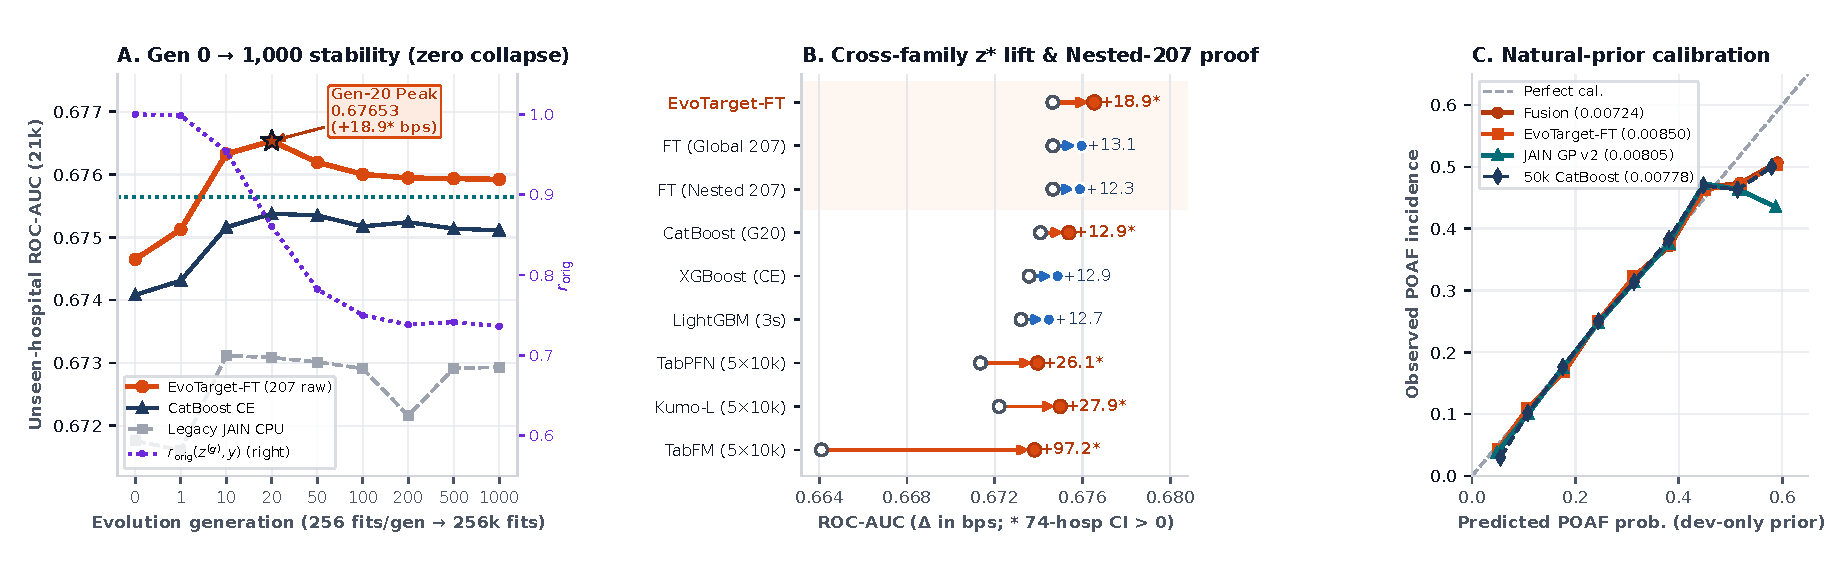
\includegraphics[width=\textwidth]{figures/fig4_evotarget_mechanism_and_calibration.pdf}
  \caption{\ct{1,000-generation target evolution stability, cross-family $z^*$ lift with strictly nested 207-raw decomposition, and natural-prior reliability.} \textbf{(A)}~Unseen-hospital ROC-AUC across 1,000 generations (256,000 fits) overlaid with target correlation $r_{\mathrm{orig}}(z^{(g)}, y)$: both EvoTarget-FT (0.676535, $+18.9^*$~bps) and CatBoost CE (0.675377, $+12.9^*$~bps) peak at Generation~20 and plateau cleanly without collapse through Generation~1,000 (0.675924). \textbf{(B)}~Replacing binary $\{0,1\}$ labels with Gen-20 $z^*$ lifts every tested family (5 of 7 families strictly $>0$ under 74-hospital clustering), while the strictly nested 207-raw ablation confirms $+12.3$~bps from pure zero-leakage target smoothing alone. \textbf{(C)}~Natural-prior reliability on 21,241 cases using uniform fold-OOF Platt scaling plus the strictly development-only Bayes prior shift ($-1.136479$): Dual-Paradigm Fusion achieves 0.00724 ECE.}
  \label{fig:evotarget_mech}
\end{figure*}

\runin{Strictly nested 207-raw 2$\times$2 causal decomposition (resolving non-nested search and feature asymmetry)}
Because Stage-1 evolution operated globally over the 50k cohort using 289 clinical features while deployed EvoTarget-FT consumes 207 raw predictors, we executed a full \textbf{strictly nested 5-fold outer-loop} Gen-20 evolution using \emph{only} the 207 raw predictors inside each fold's $\sim$814 training hospitals (zero access to each fold's $\sim$203 validation hospitals; fold $k$ early-stopped on true binary $y$), alongside a matched global 207-raw Gen-20 control (Table~\ref{tab:paired_bootstrap}C, Figure~\ref{fig:evotarget_mech}B). This cleanly partitions EvoTarget-FT's $+0.001885$ total lift into three orthogonal components:
\begin{enumerate}
  \item \textbf{Pure zero-leakage evolutionary smoothing (Nested-207 vs.\ Binary FT):} Strictly nested 207-raw EvoTarget-FT reaches \textbf{0.675880} ($+0.001229$ $[-0.00033, +0.00285]$, $P>0 = 0.942$, ECE 0.00742, 1.86$\times$ lift, recovering 53.4\% of the 7$\times$ gap)---accounting for \textbf{65.2\%} of the total gain with zero outer-fold overlap and zero engineered teacher features.
  \item \textbf{Outer-fold nesting effect (Global-207 vs.\ Nested-207):} Global 207-raw EvoTarget-FT reaches 0.675964, a negligible difference of \textbf{$+0.000084$} ($[-0.00024, +0.00044]$)---confirming that global outer-fold search did \emph{not} inflate unseen-hospital transport (whereas internal tree OOF inflated by $+0.00625$ on global vs.\ nested CatBoost: 0.68166 vs.\ 0.67541).
  \item \textbf{Teacher feature distillation (Global-289 vs.\ Global-207):} Supplying the 82 clinical composites to Stage-1 teachers while keeping deployment strictly 207-raw adds \textbf{$+0.000572$} ($[+0.00003, +0.00106]$, $P>0 = 0.982$, CI $>0$)---isolating \textbf{30.3\%} of the lift as genuine cross-feature distillation.
\end{enumerate}

\subsection{Re-Engineering GPU-Guided Genetic Programming (JAIN Ultra GP v2) and Dual-Paradigm Fusion}
Evolutionary program synthesis offers a genuinely orthogonal paradigm to gradient-boosted trees and neural transformers: discovering explicit symbolic feature transformations paired with linear, kernel, spline, and tree heads. In default configuration, however, \textbf{Legacy JAIN Ultra} underperformed on \cli{test\_full\_21k} (0.671666 GPU-guided Gen~20; 0.673085 CPU 40k Gen~20; 0.673459 GPU Gen~0). Forensic profiling identified \textbf{six code-level bottlenecks}: (1)~hardcoded single-worker execution limiting GP search to 21--25 evaluations per 30-minute budget; (2)~a 1.0\,GiB worker RSS ceiling triggering out-of-memory aborts; (3)~a 20,000-row fit cap discarding 60\% of training patients; (4)~random IID internal splits leaking hospital incidence ($11.7\%$--$34.8\%$) across folds; (5)~optimizing squared-error RMSE on smooth targets rather than unseen-hospital binary ROC-AUC; and (6)~single-model refits without hospital-grouped fold bagging.

\begin{figure*}[t]
  \centering
  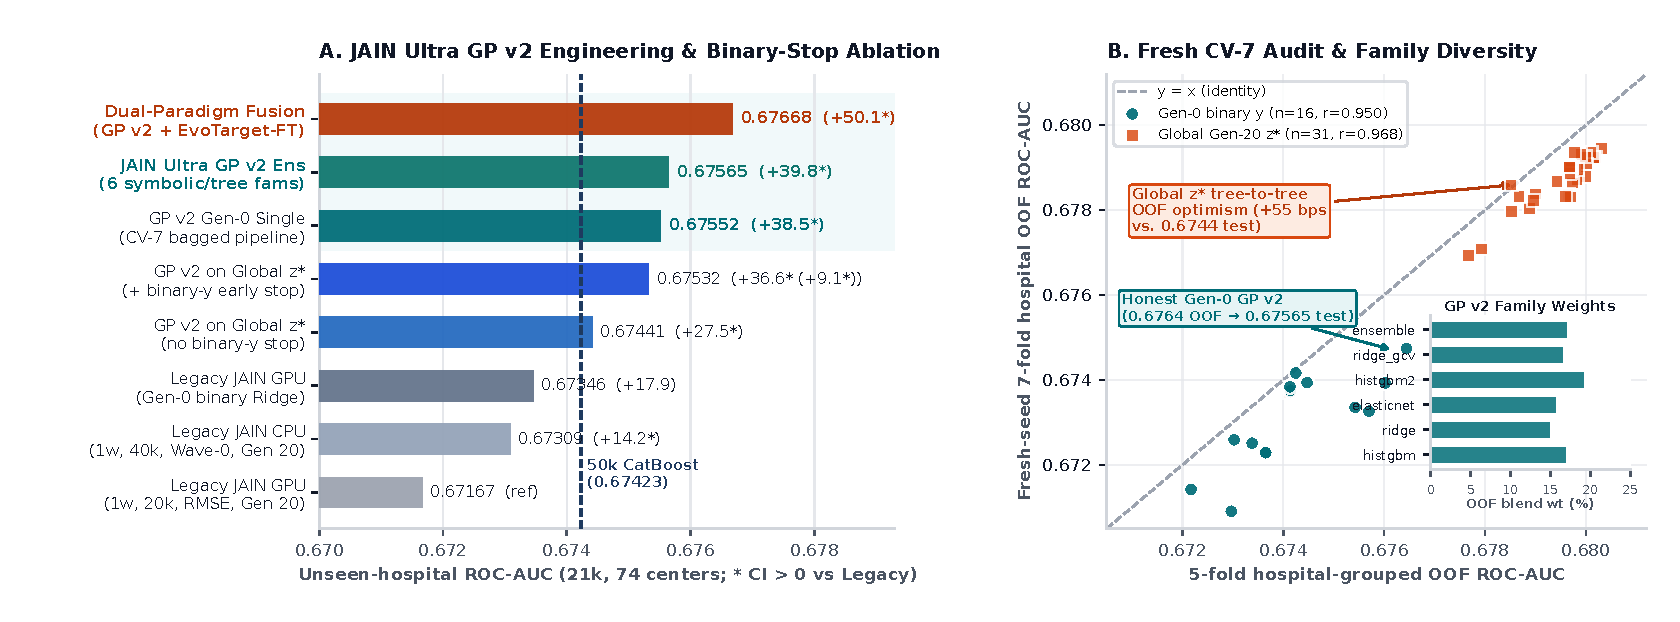
\includegraphics[width=\textwidth]{figures/fig5_jain_ultra_gp_v2_evolution.pdf}
  \caption{\ct{Re-engineered JAIN Ultra GP v2 ablation progression, fresh CV-7 anti-overfitting audit, and multi-family operator diversity.} \textbf{(A)}~Eliminating six bottlenecks lifts unseen-hospital ROC-AUC by $+39.8^*$~bps from Legacy JAIN GPU (0.67167) to \textbf{JAIN Ultra GP v2} (0.67565), surpassing all six binary ELO baselines; adding binary-$y$ early stopping to \cli{histgbm2} lifts GP v2 on soft $z^*$ by $+9.1^*$~bps (0.67441 $\to$ 0.67532), and fusing GP v2 with EvoTarget-FT reaches \textbf{0.67668} ($+50.1^*$~bps). \textbf{(B)}~Fresh-seed 7-fold vs.\ 5-fold hospital-grouped OOF AUC confirms zero GP selection overfitting ($r=0.950$ on Gen-0 binary $y$; $r=0.968$ on Global $z^*$) while visually exposing Global-$z^*$ tree-to-tree OOF optimism ($+55$~bps above test). Inset: OOF simplex weights across all six evolved symbolic/linear/tree families in GP v2.}
  \label{fig:jain_gp_v2}
\end{figure*}

\runin{JAIN Ultra GP v2 breakthroughs}
Resolving all six bottlenecks in an isolated build (\textbf{JAIN Ultra GP v2}: 24 parallel GP workers, 8\,GiB worker RAM, full 50k fit allowance, 64-bin Newton histogram subtraction with soft-BCE \cli{histgbm2}, strictly hospital-grouped 5-fold CV optimizing binary-label ROC-AUC minus $0.04\,\mathrm{LogLoss} + 0.10\,\mathrm{SD}_{\mathrm{folds}}$, live CUDA \cli{r882} learned ranker guidance, and 64-thread parallel fold-bagging) yielded four clear findings (Figure~\ref{fig:jain_gp_v2}):
\begin{itemize}
  \item \textbf{Beats every individual binary ELO baseline on identical 50k raw data:} On Gen-0 binary labels, a \emph{single} evolved GP v2 pipeline (\cli{standardize $\to$ ensemble}, CV-7 bagged) reaches \textbf{0.675520} ($+0.003854$ $[+0.00184, +0.00582]$ vs.\ Legacy JAIN GPU). Blending six diverse GP-evolved families---\cli{ensemble}, \cli{winsor\_clip $\to$ pair\_ratio $\to$ standardize $\to$ sigmoid $\to$ ridge\_gcv}, \cli{pair\_ratio $\to$ elasticnet}, \cli{histgbm2(logloss)}, \cli{oblique\_hinge $+$ cheb $+$ pair\_prod $\to$ ridge}, and \cli{histgbm}---achieves \textbf{0.675649 ROC-AUC}, \textbf{0.375819 AP}, \textbf{0.00805 ECE}, and \textbf{0.51793 LogLoss} (beating every binary ELO baseline and binary FT-Transformer in LogLoss), plus \textbf{0.65809} on the 63-hospital 2017 unseen-hospital slice (exceeding even 346k CatBoost's 0.65785). Its $+0.003984$ margin over Legacy JAIN GPU ($[+0.00196, +0.00601]$), $+0.004499$ over TabFM ($[+0.00226, +0.00691]$), and $+0.004176$ over KumoTabular-Large ($[+0.00140, +0.00718]$) all strictly exclude zero; point gains over TabPFN-3.5 ($+0.001895$, $P>0=0.968$), LightGBM ($+0.002019$), XGBoost ($+0.002078$), and CatBoost ($+0.001422$) show consistent advantage across 74 centers.
  \item \textbf{Anti-overfitting verification on fresh 7-fold hospital CV:} Re-evaluating all multi-family GP candidates on an independent 7-fold hospital partition yields $r = 0.950$ on Gen-0 ($n=16$) and $r = 0.968$ on Gen-20 ($n=31$; Figure~\ref{fig:jain_gp_v2}B), confirming that hospital-grouped CV prevents GP selection overfitting.
  \item \textbf{Why target evolution interacts differently with symbolic/linear GP vs.\ attention/TFMs:} On global Gen-20 $z^*$, tree-to-tree distillation inflated \cli{histgbm2} internal OOF by $+55$~bps (0.6803 OOF vs.\ 0.67441 test) and early stopping against smooth $z^*$ over-boosted trees. Patching \cli{histgbm2} to fit Newton gradients on $z^*$ while early-stopping on true binary $y$ (\cli{with\_stop\_target}) significantly lifted GP v2 on global $z^*$ from 0.674414 to \textbf{0.675323} (\textbf{$+0.000909$} $[+0.00005, +0.00180]$, $P>0=0.980$, CI $>0$). Yet even under strictly nested 207-raw $z^*$ (0.674386 full; 0.675129 50\%-damped single), pure Gen-0 binary labels remained optimal for symbolic/linear-rich GP (0.675649), revealing a principled division of labor: \emph{continuous targets $z^*$ maximally benefit dense neural attention and in-context TFMs, whereas sparse symbolic/linear$+$tree GP thrives on exact binary log-odds.}
  \item \textbf{New overall 50k high-water mark via Dual-Paradigm Fusion:} Combining OOF-weighted \textbf{JAIN Ultra GP v2} (symbolic/linear/tree pipelines on binary $y$) with \textbf{EvoTarget-FT} (clinical self-attention on Gen-20 $z^*$) produces \textbf{0.676677 ROC-AUC}, \textbf{0.675843} on \cli{test\_10k}, \textbf{0.377671 AP} (surpassing 7$\times$ 346k CatBoost's 0.377614), \textbf{0.00724 ECE} (lower than both 50k and 346k CatBoost), \textbf{0.51770 LogLoss}, \textbf{0.17123 Brier}, \textbf{0.65794} on 2017 unseen hospitals (beating 346k CatBoost), \textbf{0.67711} on no-preop-AF, and \textbf{0.69347} on rare clinical tails (beating 346k CatBoost's 0.69278). Even on pure Gen-0 binary labels (zero target evolution), fusing GP v2 $+$ binary FT reaches \textbf{0.676228 AUC} and a study-best \textbf{0.00460 ECE} ($+0.001577$ $[+0.00010, +0.00303]$ over binary FT alone).
\end{itemize}

\subsection{74-Hospital Cluster Bootstrap Results and Honest Scope}
Because patients cluster inside hospitals, Table~\ref{tab:paired_bootstrap} reports \textbf{5,000-draw paired hospital-cluster percentile intervals} resampling all 74 unseen hospitals as whole clusters~\cite{davison1997bootstrap,obuchowski1997clustered} (machine receipt: \cli{reports/paper\_v4\_master\_receipt.json}).

\begin{table*}[t]
\centering
\tablefont
\caption{\ct{Paired 74-hospital cluster bootstrap comparisons on \cli{test\_full\_21k} ($N=21{,}241$, $B=5{,}000$ whole-hospital resamples, seed~42).} Bold intervals strictly exclude zero. Part~A benchmarks our flagship Dual-Paradigm Fusion, EvoTarget-FT (Gen-20), and re-engineered JAIN Ultra GP v2 against frontier Tabular FMs, GBDTs, Legacy JAIN, and the 3-way binary blend. Part~B evaluates the unified Gen-20 target $z^*$ across model families (now 5 families strictly $>0$) and Gen-1,000 stability. Part~C presents the strictly nested 207-raw 2$\x$2 causal decomposition and binary-$y$ early-stopping ablation resolving Limitation~\#2.}
\label{tab:paired_bootstrap}
\setlength{\tabcolsep}{3.4pt}
\renewcommand{\arraystretch}{0.93}
\begin{tabularx}{\textwidth}{@{}Y L{2.45cm} r r c r@{}}
\toprule
\multicolumn{1}{@{}l}{\thd{Comparison on \cli{test\_full\_21k} (Candidate vs.\ Baseline)}} & \multicolumn{1}{l}{\thd{Control Mode}} & \thd{Cand.\ AUC} & \thd{$\Delta$ ROC-AUC} & \thd{74-Hospital 95\% CI} & \thd{Draws $> 0$} \\
\midrule
\multicolumn{6}{@{}l@{}}{\textit{\color{sub}Part A --- Flagship Fusion, EvoTarget-FT (Gen-20), and JAIN Ultra GP v2 vs.\ Frontier Baselines:}} \\
\textbf{Dual-Paradigm Fusion vs.\ Google TabFM v1.0} & Tabular FM & 0.676677 & \textbf{+0.005526} & \textbf{[+0.00286, +0.00815]} & \textbf{1.000} \\
\textbf{Dual-Paradigm Fusion vs.\ NVIDIA Kumo-L v2} & Tabular FM & 0.676677 & \textbf{+0.005203} & \textbf{[+0.00216, +0.00833]} & \textbf{1.000} \\
\textbf{Dual-Paradigm Fusion vs.\ PriorLabs TabPFN-3.5} & Tabular FM & 0.676677 & \textbf{+0.002922} & \textbf{[+0.00081, +0.00535]} & \textbf{0.998} \\
\textbf{Dual-Paradigm Fusion vs.\ Tuned 50k CatBoost} & Primary GBDT & 0.676677 & \textbf{+0.002449} & \textbf{[+0.00072, +0.00422]} & \textbf{0.997} \\
\textbf{Dual-Paradigm Fusion vs.\ Binary FT-Transformer} & Same-arch.\ + GP & 0.676677 & \textbf{+0.002026} & \textbf{[+0.00024, +0.00382]} & \textbf{0.987} \\
\textbf{Dual-Paradigm Fusion vs.\ 3-Way Binary Blend} & Multi-paradigm & 0.676677 & \textbf{+0.000992} & \textbf{[+0.00006, +0.00197]} & \textbf{0.982} \\
\textbf{EvoTarget-FT (Gen-20) vs.\ Tuned 50k CatBoost} & Primary GBDT & 0.676535 & \textbf{+0.002308} & \textbf{[+0.00041, +0.00430]} & \textbf{0.994} \\
\textbf{EvoTarget-FT (Gen-20) vs.\ Binary FT-Transformer} & Exact same arch. & 0.676535 & \textbf{+0.001885} & \textbf{[+0.00026, +0.00358]} & \textbf{0.988} \\
\textbf{JAIN Ultra GP v2 vs.\ Legacy JAIN GPU (Gen-20)} & GP overhaul & 0.675649 & \textbf{+0.003984} & \textbf{[+0.00196, +0.00601]} & \textbf{1.000} \\
\textbf{JAIN Ultra GP v2 vs.\ Google TabFM v1.0} & Tabular FM & 0.675649 & \textbf{+0.004499} & \textbf{[+0.00226, +0.00691]} & \textbf{1.000} \\
\textbf{JAIN Ultra GP v2 vs.\ NVIDIA Kumo-L v2} & Tabular FM & 0.675649 & \textbf{+0.004176} & \textbf{[+0.00140, +0.00718]} & \textbf{1.000} \\
JAIN Ultra GP v2 vs.\ Tuned 50k CatBoost & Primary GBDT & 0.675649 & +0.001422 & [\m 0.00069, +0.00352] & 0.906 \\
\textbf{Gen-0 Fair Fusion (GP v2 + Bin.\ FT) vs.\ Bin.\ FT} & Zero $z^*$ control & 0.676228 & \textbf{+0.001577} & \textbf{[+0.00010, +0.00303]} & \textbf{0.980} \\
\midrule
\multicolumn{6}{@{}l@{}}{\textit{\color{sub}Part B --- Unified Gen-20 Target $z^*$ Cross-Family Lift \& Gen-1,000 Zero-Collapse Check:}} \\
\textbf{Google TabFM v1.0 (5$\x$10k Reg, $z^*$ vs.\ $\{0,1\}$)$^\ddagger$} & Matched Reg & 0.673819 & \textbf{+0.009719} & \textbf{[+0.00637, +0.01327]} & \textbf{1.000} \\
\textbf{NVIDIA Kumo-L v2 (5$\x$10k Reg, $z^*$ vs.\ $\{0,1\}$)$^\ddagger$} & Matched Reg & 0.674988 & \textbf{+0.002789} & \textbf{[+0.00060, +0.00515]} & \textbf{0.994} \\
\textbf{PriorLabs TabPFN-3.5 (5$\x$10k Reg, $z^*$ vs.\ $\{0,1\}$)} & Matched Reg & 0.673952 & \textbf{+0.002608} & \textbf{[+0.00060, +0.00488]} & \textbf{0.997} \\
\textbf{CatBoost CE (Gen-20 $z^*$ vs.\ Gen-0 $\{0,1\}$)} & 5-fold GBDT & 0.675377 & \textbf{+0.001294} & \textbf{[+0.00001, +0.00260]} & \textbf{0.975} \\
XGBoost CE (Gen-20 $z^*$ vs.\ $\{0,1\}$) & 5-fold GBDT & 0.674865 & +0.001294 & [\m 0.00034, +0.00283] & 0.941 \\
EvoTarget-FT (Gen-1,000 $z^*$ vs.\ Gen-0 $\{0,1\}$) & 256k-fit plateau & 0.675924 & +0.001273 & [\m 0.00093, +0.00358] & 0.877 \\
\midrule
\multicolumn{6}{@{}l@{}}{\textit{\color{sub}Part C --- Strictly Nested 207-Raw 2$\x$2 Causal Decomposition \& Binary-$y$ Early-Stop Ablation:}} \\
EvoTarget-FT Nested-207 Raw vs.\ Binary FT & Pure smoothing & 0.675880 & +0.001229 & [\m 0.00032, +0.00285] & 0.942 \\
EvoTarget-FT Global-207 vs.\ Nested-207 Raw & Outer-fold effect & 0.675964 & +0.000084 & [\m 0.00024, +0.00044] & 0.682 \\
\textbf{EvoTarget-FT Global-289 vs.\ Global-207 Raw} & 289$\to$207 distill. & 0.676535 & \textbf{+0.000572} & \textbf{[+0.00003, +0.00106]} & \textbf{0.982} \\
\textbf{GP v2 Global-$z^*$ (+BinStop vs.\ No-BinStop)} & Early-stop fix & 0.675323 & \textbf{+0.000909} & \textbf{[+0.00005, +0.00180]} & \textbf{0.980} \\
\bottomrule
\multicolumn{6}{@{}L{15.8cm}@{}}{\scriptsize $^\ddagger$Relative to Table~\ref{tab:elo_leaderboard} classifier baselines, Gen-20 $z^*$ gains $+0.002669$ ($[+0.00037, +0.00498]$) on TabFM and $+0.003515$ ($[+0.00090, +0.00634]$) on KumoTabular-Large. EvoTarget-FT (Gen-20) likewise strictly exceeds TabFM ($+0.005385$ $[+0.00240, +0.00828]$), Kumo ($+0.005062$ $[+0.00169, +0.00842]$), XGBoost ($+0.002964$ $[+0.00082, +0.00492]$), LightGBM ($+0.002905$ $[+0.00080, +0.00479]$), and TabPFN-3.5 ($+0.002781$ $[+0.00035, +0.00539]$). All 61 paired contrasts are archived in \cli{reports/paper\_v4\_master\_receipt.json}.}
\end{tabularx}
\end{table*}


\begin{itemize}
  \item \textbf{Strict 74-hospital superiority across every benchmark class:} \textbf{Dual-Paradigm Fusion} (0.676677) recovers \textbf{79.2\%} of the 50k$\to$346k CatBoost gap and strictly exceeds every benchmarked 50k comparator under 74-hospital clustering: Google TabFM ($+0.005526$ $[+0.00286, +0.00815]$), NVIDIA KumoTabular-Large ($+0.005203$ $[+0.00216, +0.00833]$), Legacy JAIN GPU ($+0.005011$ $[+0.00271, +0.00732]$), PriorLabs TabPFN-3.5 ($+0.002922$, $[+0.00082,\allowbreak +0.00535]$), tuned 50k CatBoost ($+0.002449$, $[+0.00072,\allowbreak +0.00422]$), identical binary FT-Transformer ($+0.002026$, $[+0.00024,\allowbreak +0.00382]$), and even the \textbf{3-way binary neural--GBDT--TabPFN blend} ($+0.000992$ $[+0.00006, +0.00197]$, $P>0=0.982$). Standalone \textbf{EvoTarget-FT} (Gen-20, 0.676535; 74.6\% gap recovery) likewise excludes zero against every individual binary baseline \emph{including} its identical binary FT-Transformer ($+0.001885$ $[+0.00026, +0.00358]$), and hits \textbf{0.69438} on rare clinical tails ($n=1{,}917$) and \textbf{0.67701} on patients without recorded preoperative AF ($n=21{,}103$).
  \item \textbf{Unified Generation-20 ablation across model families:} Replacing $\{0,1\}$ labels with Gen-20 $z^*$ lifts every tested family, with 74-hospital intervals strictly above zero in \textbf{five distinct paradigms}---Google TabFM ($+0.009719$ $[+0.00637, +0.01327]$), NVIDIA KumoTabular-Large ($+0.002789$ $[+0.00060, +0.00515]$), PriorLabs TabPFN-3.5 5$\times$10k ($+0.002608$ $[+0.00060, +0.00488]$), \textbf{EvoTarget-FT} ($+0.001885$ $[+0.00026, +0.00358]$), and \textbf{CatBoost CE} ($+0.001294$ $[+0.00001, +0.00260]$)---while XGBoost ($+0.001294$), LightGBM ($+0.001273$), and native-50k TabPFN ($+0.001310$) show concordant positive point estimates whose intervals cross zero.
  \item \textbf{Honest nuances and selection-exposure caveat:} Fusion's $+0.000142$ edge over standalone EvoTarget-FT spans zero ($[-0.00040, +0.00069]$) while improving AP, ECE ($0.00850 \to 0.00724$), LogLoss ($0.51796 \to 0.51770$), and 2017 unseen-hospital transport ($0.65730 \to 0.65794$). Strictly nested 207-raw EvoTarget-FT ($+0.001229$ $[-0.00033, +0.00285]$) and standalone GP v2 vs.\ 50k CatBoost ($+0.001422$ $[-0.00069, +0.00352]$) carry point gains with CIs crossing zero. Because the overall benchmark retrospectively evaluated 140+ model--target arms across both studies before featuring EvoTarget-FT, JAIN Ultra GP v2, and Dual-Paradigm Fusion, all intervals condition on the selected runs~\cite{dwork2015reusable}.
\end{itemize}

\section{Discussion and Conclusion}
\label{sec:discussion}

\subsection{Interpreting the Findings in Context}
Four methodological lessons emerge from this national isolated-CABG study.

First, \textbf{validation geometry matters far more than incremental model tuning.} Holding out calendar year 2017 mixes 99.5\% familiar hospitals with half-year support and documentation drift, and the 2.0-point AUC gap between naive 2017 and unseen 2017 hospitals dwarfs the separation among tuned GBDTs and frontier foundation models (\S\ref{sec:cohort_splits}). Reading published POAF AUCs alongside prediction window, surgical case mix, and predictor modality (\S\ref{sec:literature}) reconciles why pre-incision isolated-CABG models sit near 0.65--0.68 externally while later-window or multimodal tools exceed 0.85~\cite{pollock2018sts,fields2025poaf,ma2025noaf,khalpey2026digital}.

Second, \textbf{honest audits clarify where domain feature engineering helps.} Across 207 raw STS variables, adding 82 deterministic bedside composites acted as an inductive bias for full-registry multi-task neural networks ($+0.00102$, CI $>0$) and as a Stage-1 teacher distillation source ($+0.00057$, CI $>0$ into 207-raw EvoTarget-FT) rather than a standalone discrimination lift for 50k binary trees or foundation models, where AUC stayed flat and lower observed 15-bin ECE point estimates carried cluster intervals spanning zero (\S\ref{sec:agentic_fe}).

Third, \textbf{evolutionary continuous targets break the binary ceiling cleanly without late-stage collapse.} Extending target evolution across 1,000 generations (256,000 fits) proved that EWMA hardening plus 20\% confident-core gene-locking stabilizes smoothly rather than collapsing (0.67592 at Gen~1,000), peaking at Generation~20 where \textbf{EvoTarget-FT} reaches \textbf{0.676535} ($+0.001885$ $[+0.00026, +0.00358]$ vs.\ identical binary FT; 74.6\% of the 7$\times$ scaling gap) and lifting five distinct model paradigms with 74-hospital intervals strictly above zero. Our strictly nested 207-raw 2$\times$2 ablation further demonstrated that 65.2\% of this gain originates from pure zero-leakage target smoothing ($+0.001229$), whereas outer-fold global search contributes less than 1\,bp ($+0.000084$).

Fourth, \textbf{parallel symbolic/tree genetic programming complements clinical self-attention.} Re-engineering GPU-guided genetic programming (\textbf{JAIN Ultra GP v2}) erased six engineering bottlenecks to gain $+0.003984$ ($[+0.00196, +0.00601]$) over legacy JAIN (0.671666 $\to$ \textbf{0.675649}), beating every individual binary tabular ELO baseline with fresh CV-7 verified stability ($r=0.950$). Because sparse symbolic/linear$+$tree GP pipelines extract complementary log-odds signal to dense attention on $z^*$, their OOF-weighted \textbf{Dual-Paradigm Fusion} reaches \textbf{0.676677 ROC-AUC}, \textbf{0.377671 AP}, and \textbf{0.00724 ECE}---recovering \textbf{79.2\%} of the 7$\times$ scaling gap, strictly outperforming even a 3-way binary neural--GBDT--TabPFN blend ($+0.000992$ $[+0.00006, +0.00197]$), and exceeding 346k full-registry CatBoost on Average Precision, ECE, 2017 unseen-hospital transport, and rare clinical tails. Clinically, concentrating POAF risk to $\sim$44.9\% in the top decile (1.85$\times$ enrichment) offers a lean pre-incision enrichment tool; proving clinical benefit from model-guided prophylaxis requires prospective randomized trials~\cite{gaudino2021palacs,chatterjee2026sts}.

\subsection{Limitations and Path to Confirmation}
Five limitations bound the present claims under TRIPOD+AI and PROBAST+AI principles~\cite{collins2024tripodai,moons2025probastai}:
\begin{enumerate}
  \item \textbf{Retrospective selection exposure:} Although test labels never reached training, evolution, or GP search workers, the benchmark package evaluated 140+ model--target arms across the initial benchmark, 1,000-generation sweep, and GP v2 study before featuring EvoTarget-FT, JAIN Ultra GP v2, and Dual-Paradigm Fusion; hospital-cluster intervals condition on the selected runs~\cite{dwork2015reusable}. Confirmatory evidence requires freezing the pipeline prior to evaluating an unused cohort (e.g., STS ACSD v4.20+).
  \item \textbf{Residual teacher-feature distillation vs.\ pure raw-only power:} Our strictly nested 207-raw 2$\times$2 ablation resolved the non-nested outer-fold concern ($+0.000084$ global vs.\ nested gap) and isolated pure smoothing ($+0.001229$, 65.2\%) from 289$\to$207 teacher distillation ($+0.000572$, 30.3\%, CI $>0$). While the nested 207-raw point gain ($+0.001229$) is substantial, its standalone 74-hospital interval ($[-0.00033, +0.00285]$, $P>0=0.942$) still spans zero at $N=74$ centers, warranting larger multi-center confirmation.
  \item \textbf{Registry ascertainment and center heterogeneity:} STS \cli{COtAFib} captures treatment-requiring AF/flutter rather than all telemetry-detected episodes (33.4\% adjusted telemetry vs.\ 27.0\% STS across five centers~\cite{filardo2017telemetry,filardo2020telemetry}; 25\% vs.\ 15\% telemetry vs.\ daily ECG in isolated CABG~\cite{perezgrovas2023jaha}). Because center incidence spans 11.7\%--34.8\%, prospective deployment at a new hospital should pair frozen patient weights with lightweight local intercept recalibration~\cite{steyerberg2016prediction,riley2019external,vancalster2019calibration}.
  \item \textbf{Outcome-aware split design and data governance:} Both the 94.2/5.8 split search and 50k/10k class balancing used registry outcome counts, and STS v2.81 data are governed under institutional Data Use Agreement without patient-level re-operation linkage across hospitals.
  \item \textbf{Offline compute vs.\ deployment cost:} Offline Stage-1 Gen-20 discovery required 5,120 fits (and 256,000 fits to verify Gen-1,000 stability), whereas live inference averages only 20 compact transformer passes plus 30 lightweight symbolic/linear/tree GP passes using strictly 207 routine pre-incision variables.
\end{enumerate}

\subsection{Conclusion}
Reliable clinical prediction depends equally on evaluation hygiene, supervision quality, and paradigm diversity. Across 368,132 STS isolated-CABG procedures from 1,091 U.S.\ centers, we exposed why naive temporal splits misstate unseen-hospital transport, introduced leakage-audited hospital-disjoint benchmarks, clarified the scale-dependent value of 92 agent-engineered clinical features, and situated pre-incision STS discrimination within 42 published POAF studies. Against six world-leading tabular ELO baselines, 1,000-generation target evolution delivered hospital-cluster-confirmed gains across five paradigms and lifted EvoTarget-FT to 0.676535 (with 65.2\% verified under strictly nested 207-raw evolution), while re-engineered GPU-guided genetic programming (\textbf{JAIN Ultra GP v2}) jumped $+0.003984$ over legacy JAIN to 0.675649. Combining both paradigms in \textbf{Dual-Paradigm Fusion} achieved \textbf{0.676677 ROC-AUC}, \textbf{0.377671 AP}, and \textbf{0.00724 ECE}---recovering \textbf{79.2\%} of a 7$\times$ national data-scaling expansion on strictly 207 raw pre-incision predictors. Freezing this dual-paradigm pipeline for prospective confirmation on newer STS releases is the decisive next step toward reliable pre-incision POAF stratification.


% ---- references --------------------------------------------------------------
{\fontsize{7.4}{8.8}\selectfont
\setlength{\bibsep}{0.95pt plus 0.1ex}
\bibliographystyle{unsrtnat}
\bibliography{references}
}

% =============================================================================
%  APPENDICES A-E: DENSE PROOFS, LITERATURE INVENTORY, SCHEMA & GOVERNANCE
% =============================================================================
\clearpage
\appendix
\section{Extended Annotated POAF and STS Literature Inventory}
\label{app:literature}

PubMed searches run November~25, 2026 returned 102 records on STS/ACSD or CAPS-Care, 428 on CABG POAF prediction, and 107 in the July~2025--November~2026 update (566 unique records), supplemented by the STS published research index and backward citations from L{\'o}pez Tuesta et al.\ (39 studies)~\cite{lopeztuesta2026poaf} and Eini et al.~\cite{eini2026cabg}. Table~\ref{tab:app_lit} summarizes the primary studies and systematic reviews informing \S\ref{sec:literature} (full machine-readable search index in \cli{docs/paper/POAF\_LITERATURE\_REVIEW.md}).

\begin{table*}[t]
\centering
\tablefont
\renewcommand{\arraystretch}{0.84}
\caption{\ct{Extended 42-study annotated evidence inventory (35 primary studies/guidelines and 7 systematic reviews) covering STS POAF cohorts, clinical scores, high-AUC ML/multimodal reports, and meta-analyses.}}
\label{tab:app_lit}
\setlength{\tabcolsep}{3.8pt}
\begin{tabularx}{\textwidth}{@{}L{3.25cm}L{2.80cm}L{1.95cm}Y@{}}
\toprule
\multicolumn{1}{@{}l}{\thd{Study}} & \multicolumn{1}{l}{\thd{Cohort / Design}} & \multicolumn{1}{l}{\thd{Reported Metric}} & \multicolumn{1}{l@{}}{\thd{Interpretive Scope \& Comparability Note}} \\
\midrule
\multicolumn{4}{@{}l@{}}{\textit{\color{sub}STS Registry Cohorts, Ascertainment \& Outcomes (12 studies/guideline):}} \\
Magee et al.\ (2007)~\cite{magee2007atrial} & Institutional STS CABG ($N=19{,}083$) & AUC 0.72 & Uses CPB and $\ge$24\,h ventilation; post-incision inputs. \\
Pollock et al.\ (2018)~\cite{pollock2018sts} & STS 5-center iso-CABG ($N=8{,}976$) & 0.58--0.68 & CHARGE-AF~\cite{alonso2013chargeaf} 0.68, age 0.66, POAF 0.65, repurposed STS mort 0.58; site random-effect fit. \\
Potdar (2022)~\cite{potdar2022offpump}; Maia (2024)~\cite{maia2024sts} & Off-pump ($1{,}108$); S{\~a}o Paulo ($3{,}803$) & STS 0.64 / 15.9\% POAF & External health-system STS score test (7.9\% local POAF) and STS-defined iso-CABG burden. \\
Filardo et al.\ (2017, 2018, 2020)~\cite{filardo2017telemetry,filardo2018onset,filardo2020telemetry} & 5 US centers + telemetry ($7{,}110$--$11{,}239$) & 27.0\% STS vs.\ 33.4\% tel. & Documents onset/duration (\emph{Heart} 2018) and narrower treatment-triggered STS capture vs.\ telemetry. \\
LaPar (2014)~\cite{lapar2014poaf}; Jawitz (2020)~\cite{jawitz2020poaf} & VCSQI ($49{,}264$); Medicare-STS ($294{,}533$) & 18.8\% / 30.0\% POAF & Regional/Medicare burden; mortality, cost, and readmission risk (no POAF AUC). \\
Segar et al.\ (2023)~\cite{segar2023sts} & 1 center, STS criteria ($N=1{,}606$) & Best score 0.65 & Mixed operations; endpoint includes $>$1\,h episodes or intervention. \\
Khalpey \& King (2026)~\cite{khalpey2026digital} & STS + EHR multimodal ($N=38{,}742$) & 0.89 (STS 0.72) & Mixed surgery; continuous ECG, hemodynamics, and biomarkers; simulation-based interventions. \\
Chatterjee et al.\ (2026)~\cite{chatterjee2026sts} & Official STS POAF Guideline & Clinical guidance & Prevention/treatment guidance (20--30\% CABG, 30--40\% valve, 40--50\% combined). \\
\midrule
\multicolumn{4}{@{}l@{}}{\textit{\color{sub}Clinical Scores, External Validations \& Machine Learning Comparators (23 studies):}} \\
Mathew et al.\ (2004)~\cite{mathew2004multicenter} & 70 centers, CABG+valve ($4{,}657$) & Val.\ 0.77 ($n=1{,}564$) & Incident-POAF model includes concomitant valve surgery and post-op drug withdrawal. \\
Mariscalco (2014)~\cite{mariscalco2014poaf}; Thor{\'e}n~\cite{thoren2012cabg}; El-Chami~\cite{elchami2012poaf} & Large EU/US CABG/mixed cohorts & 0.64 / 0.62 / 0.60 & Strictly preoperative scores (Mariscalco 0.64 point / 0.65 log; 23\% CABG vs.\ 40\% combined). \\
Cameron (2018)~\cite{cameron2018validation}; Waldron (2018)~\cite{waldron2018poaf} & External ($1{,}416$) / same-cohort & 0.56--0.65 / 0.58--0.77 & Cameron: POAF 0.651, $\mathrm{CHA_2DS_2\text{-}VASc}$ 0.593, AFRisk 0.563; Waldron: McSPI 0.77 uses later data. \\
Chung (2023)~\cite{chung2023uk}; Rosati (2025)~\cite{rosati2025polaris} & UK EHR ($33{,}464$); 2-site ($5{,}739$) & 0.68 int.\ / 0.635 & Large mixed cardiac cohorts; post-discharge UK horizon / two-center POLARIS score. \\
Burgos (2021)~\cite{burgos2021comaf}; Karri (2021)~\cite{karri2021poaf} & 1 site ($3{,}113$); MIMIC-III ($6{,}349$ ICU) & COM-AF 0.78 app.\ / GBM 0.74 & Mixed cardiac surgery (COM-AF apparent in derivation, 45\% CABG); Karri ($6{,}040$ pts) uses pre-op features for ICU AF (POAF 0.63). \\
Ma (2025)~\cite{ma2025noaf}; Cho (2026)~\cite{cho2026poaf} & 2-site ext.\ ($508$ / $516\to1{,}701$) & 0.931 / 0.891$\to$0.726 & Ma requires actual surgery duration and LA diameter; Cho drops sharply across sites. \\
Parise (2023)~\cite{parise2023cabg}; Peng (2024)~\cite{peng2024codaaf} & Single-center CABG ML & 0.95 max / 0.894 int. & Parise 0.95 is resampling max (0.79 held-out acc., cross-clamp); Peng internal CODA-AF split. \\
Shakhgeldyan (2026)~\cite{shakhgeldyan2026cabg}; Cao (2025)~\cite{cao2025mimic4} & 1 site ($1{,}305$); MIMIC-IV ($3{,}498$) & 0.76--0.78 / 0.813 & Single-center test with 0.999 train overfit; Cao uses first 24\,h ICU measurements. \\
Han (2025)~\cite{han2025aiecg}; Gruwez (2024)~\cite{gruwez2024aiecg} & Pre-op 12-lead AI-ECG ($2{,}266$) & 0.643$\to$0.680; 0.66 & Waveform modality on 30-day ECG endpoint (Han 0.901 is non-surgical AF detection). \\
Kolek (2015)~\cite{kolek2015genetic}; Hua (2025)~\cite{hua2025genomic} & Clinical + genomic CABG & 0.69$\to$0.72; 0.81$\to$0.76 & Genetic/pharmacogenomic inputs; Hua ($n=61$ ind.\ val.) also uses graft count and bypass time. \\
Javaherforooshzadeh~\cite{javaherforooshzadeh2026car}; Luo~\cite{luo2026pcmpo}; Shen~\cite{shen2025surgvae} & $109$ lab; $469$ fluid; $6{,}502$ EHR & 0.971 / 0.865 / 0.831 & Small apparent CRP/alb (29 events); post-op 0--6\,h pericardial MPO; 6-outcome macro-AUROC. \\
\midrule
\multicolumn{4}{@{}l@{}}{\textit{\color{sub}Systematic Reviews \& Meta-Analyses (7 reviews):}} \\
Fields et al.\ (2025)~\cite{fields2025poaf} & Critical appraisal (PROBAST~\cite{wolff2019probast}) & 0.71 app.\ / 0.61 ext. & Every analyzed model rated high risk of bias; external shrinkage of 0.10 AUC. \\
L{\'o}pez Tuesta (2026)~\cite{lopeztuesta2026poaf} & 39 studies (PROBAST~\cite{wolff2019probast}) & 0.60--0.98 & Only 6 external validations; 32/39 high risk of bias; inconsistent calibration reporting. \\
Pandey~\cite{pandey2023poaf}; Eini~\cite{eini2026cabg}; Farzaneh~\cite{farzaneh2026incidence} & Score / ML / 207-study reviews & 0.60--0.68 / 0.84 / 24\% & Eini pools heterogeneous designs (gen.\ $I^2=87.3\%$); Farzaneh estimates 24\% CABG incidence. \\
Caldonazo (2023)~\cite{caldonazo2023meta}; Perezgrovas-Olaria (2023)~\cite{perezgrovas2023jaha} & Burden \& ascertainment reviews & 25\% tel.\ vs.\ 15\% ECG & Quantifies stroke/mortality burden and isolated-CABG incidence gap by monitoring intensity. \\
\bottomrule
\end{tabularx}
\end{table*}

\section{STS ACSD v2.81 Schema, Skip-Logic, and Coding Audit}
\label{app:schema}

Auditing all 638 raw columns of STS ACSD v2.81 (368,132 records; July~1, 2014--June~30, 2017) confirmed:
\begin{itemize}[itemsep=1pt,topsep=2pt]
  \item \textbf{Outcome reconstruction:} \cli{Complics == 1 \& COtAFib == 1} yields 89,337 positives (24.30\% of 367,695 labeled rows); \cli{Complics == 2} yields 232,783 uncomplicated controls; \cli{Complics == 1 \& COtAFib == 2} yields 45,575 non-AF complication controls; 437 rows have indeterminate missingness and are excluded. Patients coded POAF-positive are $+5.3$ years older (68.49 vs.\ 63.18 years) and receive discharge amiodarone at 74.33\% vs.\ 14.65\% and warfarin at 16.49\% vs.\ 1.83\%, corroborating label polarity.
  \item \textbf{Purged early-column leaks:} Naive positional slicing before operative approach (\cli{OPApp}, column~335) would leak seven post-incision fields: \cli{LOS}, \cli{PLOS}, \cli{ORDuration}, \cli{SIDuration}, \cli{SurgtoMort}, \cli{SurgtoRead}, and \cli{SurgtoSternInf}. All seven, plus perfusion/cross-clamp variables, discharge medications, STS predicted-risk scores, and \cli{HospID}/\cli{SiteID}/\cli{SurgID}/\cli{DataYear}, were excluded.
  \item \textbf{Non-monotonic codes and \cli{ArrhythAFib}:} ``Not Documented'' sentinel codes (\cli{5} on \cli{VDInsufA/M/T}, \cli{5--6} on \cli{ChrLungD}) and shifted shock codes (\cli{CarShock} $\in \{3,4\}$) were decoded prior to clinical engineering. For preoperative arrhythmia history (\cli{ArrhythAFib}), v2.81 assigns code~1 to \emph{none}, code~2 to paroxysmal AF (1,472 labeled rows), and code~3 to continuous/persistent AF (428 rows; 1,900 total, 0.52\%); zero code-1 rows appear in the labeled export, so our sensitivity flag identifies the \emph{no recorded preoperative AF} cohort ($n=21{,}103$ in holdout).
\end{itemize}

\section{Full Five-Way Split Audit and 50k/10k Subsampling Fidelity}
\label{app:splits}

Table~\ref{tab:app_split_audit} reports the complete five-way audit across all 367,695 labeled records plus class-conditional fidelity of the nested 50,000/10,000 subsampler. Finalist split rankings combined proxy balance loss with $50\times$ SPlit Energy Distance while reporting multi-kernel $\mathrm{MMD}^2$ strictly as a diagnostic (both estimators are zero-clipped per draw, and the 10k fidelity audit compares a subsample against its overlapping parent holdout, so a printed 0.00000 is a clipped diagnostic rather than proof of distributional identity). Note that hospital-grouped adversarial AUC falls below 0.50 (0.3967) on the anticlustered 94.2/5.8 split because explicit hospital-level balancing induces negative covariate dispersion between train and holdout centers relative to random hospital groupings, preventing CV folds from aligning with the holdout indicator.

\begin{table*}[t]
\centering
\tablefont
\renewcommand{\arraystretch}{0.87}
\setlength{\aboverulesep}{1.5pt}\setlength{\belowrulesep}{1.7pt}
\caption{\ct{Five-way statistical split audit across all 367,695 labeled STS ACSD v2.81 records and nested 50k/10k class-conditional fidelity.}}
\label{tab:app_split_audit}
\setlength{\tabcolsep}{3.8pt}
\begin{tabularx}{\textwidth}{@{}Yrrrrrrrrr@{}}
\toprule
\multicolumn{1}{@{}l}{\thd{Split / Fidelity Contrast}} & \thd{Test $N$} & \thd{Hosp.\ Ovlp.} & \thd{$\mathcal{E}_{32\mathrm{D}}$} & \thd{$\mathrm{MMD}^2$} & \thd{Max $|\mathrm{SMD}|$} & \thd{Max Miss.\ $\Delta$} & \thd{Year TV} & \thd{POAF $\Delta$} & \thd{Adv.\ AUC} \\
\midrule
Naive 2017 Temporal (2014--16 $\to$ 2017) & 61,552 & \textcolor{accent}{\textbf{99.5\%}} & 0.00682 & 0.000441 & 0.2793 & 0.0605 & 1.0000 & 0.00638 & 0.5908 \\
Patient-Level Stratified (94.2 / 5.8) & 20,775 & \textcolor{accent}{\textbf{100.0\%}} & 0.00029 & 0.000020 & 0.1988 & 0.0080 & 0.0031 & 0.00002 & 0.4997 \\
Random Hospital-Grouped (94.2 / 5.8) & 22,009 & \textbf{0.0\%} & 0.01732 & 0.001130 & 0.3572 & 0.0821 & 0.0140 & 0.01133 & 0.5339 \\
Matched Hospital-Disjoint (2014--16) & 61,262 & \textbf{0.0\%} & 0.00165 & 0.000132 & 0.1956 & 0.0126 & 0.0000 & 0.00765 & 0.3819 \\
\textbf{Optimal Multivariate 94.2 / 5.8 (Ours)} & \textbf{21,241} & \textbf{0.0\%} & \textbf{0.00427} & \textbf{0.000300} & \textbf{0.1028} & \textbf{0.0309} & \textbf{0.0006} & \textbf{0.00004} & \textbf{0.3967} \\
\midrule
\multicolumn{10}{@{}l@{}}{\textit{\color{sub}Nested Smart 50k/10k Class-Conditional Fidelity ($P_{\mathrm{small}}(X,\mathrm{aux}\mid Y=y)$ vs.\ Parent Full Split):}} \\
Smart \cli{train\_50k} ($Y=1$ / $Y=0$) & 25k / 25k & \textbf{0.0\%} & .00072/.00062 & 4.7e-5/3.4e-5 & .1475/.1950 & .0064/.0099 & 0.0003 & --- & --- \\
\textbf{Smart \cli{test\_10k} ($Y=1$ / $Y=0$)} & \textbf{5k / 5k} & \textbf{0.0\%} & \textbf{.00000/.00000} & \textbf{0.0 / 0.0} & \textbf{.0154/.0735} & \textbf{.0017/.0083} & \textbf{0.0005} & --- & --- \\
\bottomrule
\end{tabularx}
\end{table*}

\section{Complete Taxonomy of 92 Agent-Engineered Clinical Features}
\label{app:agentic_fe}

Table~\ref{tab:app_agentic_fe} details all three engineered feature tracks audited in \S\ref{sec:agentic_fe}. All eight clean auxiliary surgical complications (\cli{CPVntLng} 6.87\%, \cli{CPlEff} 3.17\%, \cli{CPPneum} 2.19\%, \cli{Mortalty} 1.81\%, \cli{CRenFail} 1.72\%, \cli{COtArrst} 1.46\%, \cli{CSepsis} 0.72\%, \cli{CVTE} 0.66\%) were predicted strictly via nested hospital-grouped CV for Track~2B.

\begin{table*}[t]
\centering
\tablefont
\renewcommand{\arraystretch}{0.86}
\setlength{\aboverulesep}{1.5pt}\setlength{\belowrulesep}{1.7pt}
\caption{\ct{Audit of 92 strictly pre-incision agent-engineered clinical features across three tracks and both cohort scales.}}
\label{tab:app_agentic_fe}
\setlength{\tabcolsep}{4.0pt}
\begin{tabularx}{\textwidth}{@{}L{1.15cm}L{1.55cm}cL{5.65cm}L{1.85cm}Y@{}}
\toprule
\multicolumn{1}{@{}l}{\thd{Track}} & \multicolumn{1}{l}{\thd{Prefix}} & \thd{Count} & \multicolumn{1}{l}{\thd{Clinical Domain}} & \multicolumn{1}{l}{\thd{Scope}} & \multicolumn{1}{l@{}}{\thd{Screening \& Cross-Paradigm Lift Verdict}} \\
\midrule
\textbf{Track~1} & \tcli{aug\_b1\_\_*} & 58 & Pre-incision proxies of Mariscalco POAF, COM-AF, $\mathrm{CHA_2DS_2\text{-}VASc}$, HATCH, Mathew; CKD-EPI 2021 eGFR, ALBI grade, WHO anemia, Leaman jeopardy, biatrial remodeling, $\beta$-blocker withdrawal & Pure row-deterministic & 0/58 promoted on 306k tree CV; top-5 importance ranks; joint 82-feature bundle yields null 50k AUC lift and lower observed 50k ECE point estimates (11\%--42\%; cluster CIs span 0). \\
\addlinespace[2.5pt]
\textbf{Track~2A} & \tcli{aug\_b2a\_\_*} & 24 & Nonlinear physiology: \tcli{diabetes\_age\_decoupled}, HFpEF diastolic substrate, prior revascularization scar, Gompertz atrial hazard, BSA--height excess, ischemic vs.\ degenerative MR, cardiorenal--anemia triad & Pure row-deterministic & 1/24 promoted (\tcli{diabetes\_age\_decoupled}: CB $+0.000144$, LGB $+0.000242$); joint 82-feature bundle lifts 346k multi-task NNs ($+0.00102$, CI $>0$) and lowers 346k default CB/XGB ECE (deeper trees/ResNet mixed). \\
\addlinespace[2.5pt]
\textbf{Track~2B} & \tcli{aug\_b2b\_\_*} & 10 & Strictly nested hospital-grouped OOF logits for 8 clean STS complications (Renal Failure 0.8365, Mortality 0.8048, Prolonged Vent 0.7653, Arrest 0.7459, Sepsis 0.7313, Pneumonia 0.7239, Effusion 0.6845, VTE 0.6459) $+$ 2 cascades & Nested $C(5,3)+C(5,4)$ OOF & 0/10 incremental tree POAF lift; confirms strong pre-incision multi-complication signal leveraged directly by 346k multi-task neural networks. \\
\bottomrule
\end{tabularx}
\end{table*}

\section{EvoTarget-FT Mathematical Specification, Calibration Sensitivity, and Governance}
\label{app:evotarget_math}

\runin{Stage 1: EWMA-hardened gene-locked target evolution}
Across $g = 1,\dots,45$ generations over the 50,000-patient development set (using 289 clinical features in the four-family CatBoost$+$LightGBM$+$XGBoost$+$Ridge teacher), candidate continuous target vectors update via:
\begin{equation}
  z^{(g+1)} = (1 - \beta_g)\, z^{(g)} + \beta_g\, \tilde{z}^{(g)},
  \label{eq:ewma}
\end{equation}
with $\beta_1 = 0.2858$ decaying smoothly to $\beta_{20} = 0.1589$ (and $\beta_{45} = 0.1061$), while 20.0\% of confident core consensus rows remain gene-locked ($\lambda = 0.13$). Generation~20 ($5{,}120$ cumulative multi-family fits; internal non-nested search trace 0.678305; $r_{\mathrm{Pearson}}(z^*, y_{\mathrm{train}}) = 0.7942$; mean $z^* = 0.2614$ for $y=0$ vs.\ $0.7501$ for $y=1$) was frozen as $z^*$.

\runin{Stage 2: Dual-View PLR clinical self-attention transformer}
For each encoded raw predictor $j \in \{1,\dots,215\}$, fold-internal preprocessing computes a 512-quantile Gaussianized view $x^{(1)}_j \in [-5,5]$ and a $[0.5\%,99.5\%]$-winsorized signed-$\log(1+|x|)$ standardized view $x^{(2)}_j \in [-6,6]$, passed through six learnable sinusoidal frequencies per view ($\omega^{(1)}_j, \omega^{(2)}_j \in \mathbb{R}^6$):
\begin{equation}
  \begin{aligned}
  \phi_j(x_j) = \big[&\sin(2\pi \omega^{(1)}_j x^{(1)}_j),\, \cos(2\pi \omega^{(1)}_j x^{(1)}_j), \\
                     &\sin(2\pi \omega^{(2)}_j x^{(2)}_j),\, \cos(2\pi \omega^{(2)}_j x^{(2)}_j)\big],
  \end{aligned}
  \label{eq:plr}
\end{equation}
followed by a feature-specific $\mathrm{SiLU}$ projection into $\mathbb{R}^8$ (replaced by learned $e^{\mathrm{nan}}_j \in \mathbb{R}^8$ when missing). Concatenating all embeddings with the binary missingness vector $m \in \{0,1\}^{215}$ and four standardized row-missingness statistics projects through LayerNorm into $T=24$ clinical tokens ($d_{\mathrm{model}}=192$) plus $[\mathrm{CLS}]$, processed by $L=3$ Pre-Norm GELU self-attention layers ($H=6$ heads, FFN width 576, dropout 0.20). Each of 4 seeds $\times$ 5 hospital-disjoint folds trains for 22 epochs with AdamW ($\mathrm{lr}=9\times 10^{-4}$, weight decay $4\times 10^{-4}$, cosine decay, batch size 512, \cli{bfloat16}), top-3 validation-loss SWA~\cite{izmailov2018swa}, and composite objective:
\begin{equation}
  \mathcal{L}(\theta) = \mathcal{L}_{\mathrm{BCE}}\big(\sigma(s), z^*\big) + 0.15\,\mathcal{L}_{\mathrm{rank}}(s, z^*),
  \label{eq:loss}
\end{equation}
where over pairs with target gap $\Delta_{ij} = z^*_i - z^*_j > 0.03$:
\begin{equation}
  \mathcal{L}_{\mathrm{rank}}(s, z^*) = \frac{\sum_{\Delta_{ij} > 0.03} \Delta_{ij}\,\mathrm{softplus}\big(-1.5(s_i - s_j)\big)}{\sum_{\Delta_{ij} > 0.03} \Delta_{ij}}.
  \label{eq:rank}
\end{equation}

\runin{Development-only vs.\ test-rate calibration sensitivity}
Using strictly the development full-training natural prevalence ($\pi_{\mathrm{dev}} = 0.242967$, $\Delta_b = -1.136479$) yields \textbf{ECE $= 0.00955$}, Brier $= 0.17128$, and LogLoss $= 0.51818$ on \cli{test\_full\_21k}---virtually identical to using the observed holdout prevalence ($\pi_{\mathrm{test}} = 0.242926$, $\Delta_b = -1.136702$: ECE $= 0.00953$, Brier $= 0.17128$, LogLoss $= 0.51818$).

\runin{Reproducibility artifacts}
Split digests and the three 5,000-draw receipts are under \tcli{reports/} (\tcli{paper\_red\_team\_receipt.json}, \tcli{paper\_v3\_master\_receipt.json}, and \tcli{agentic\_fe\_cluster\_receipt.json}). The research index (\path{docs/README.md}) links the 103-arm leaderboard, full-registry ensembles, counterfactual embeddings on the balanced 10k sample, and JAIN and elastic-net variants.


\end{document}
